%\documentclass{svjour3}                     % onecolumn (standard format)
\documentclass[smallcondensed]{svjour3}    % onecolumn (ditto)
%\documentclass[smallextended]{svjour3}     % onecolumn (second format)
%\documentclass[twocolumn]{svjour3}         % twocolumn
%
%\smartqed  % flush right qed marks, e.g. at end of proof
%
%\usepackage{graphicx}
\usepackage{bm}
\usepackage{mathptmx}
\usepackage{amsmath,amssymb}
%\usepackage{comments}
\usepackage{listings}
\usepackage{array}
\lstset{numbers=left,numberblanklines=false,basicstyle=\ttfamily\footnotesize,%
numberbychapter=false,columns=fullflexible,keepspaces=true}
\usepackage{slashbox}
\usepackage{natbib}
\usepackage{hyperref}
\usepackage{url}
\usepackage{tikz}
\usetikzlibrary{arrows,chains,positioning,automata,decorations,shapes,calc,matrix,fit,backgrounds} % CHECK!!
\newcommand{\gringo}{\textit{gringo}}
\newcommand{\clasp}{\textit{clasp}}
\newcommand{\clingo}{\textit{clingo}}
\newcommand{\asprin}{\textit{asprin}}
\newcommand{\asap}{\textit{teaspoon}}
\newcommand{\piclasp}{\textit{piclasp}}

\newcommand{\code}[1]{\lstinline[basicstyle=\ttfamily]{#1}}

\newcommand{\lw}[1]{\smash{\lower1.ex\hbox{#1}}}
\newcommand{\llw}[1]{\smash{\lower3.ex\hbox{#1}}}

%\newcommand{\dataCL}[5]{%
%  \code{#1} & #3 & #5 & #4
%}
%\newcommand{\dataCS}[5]{%
%  #3 & #5 & #4
%}

\newenvironment{tableC}{%
  \scriptsize
  \tabcolsep = 0.6mm
  \begin{tabular}[t]{l|rlr|rlr|rlr|rlr|rlr}\hline
    \multicolumn{1}{l|}{\llw{Instance}} &
    \multicolumn{3}{c|}{UD1} &
    \multicolumn{3}{c|}{UD2} &
    \multicolumn{3}{c|}{UD3} &
    \multicolumn{3}{c|}{UD4} &
    \multicolumn{3}{c}{UD5} \\
    & 
    \multicolumn{1}{c}{Best} & & \multicolumn{1}{c|}{\emph{tea-}} & 
    \multicolumn{1}{c}{Best} & & \multicolumn{1}{c|}{\emph{tea-}} & 
    \multicolumn{1}{c}{Best} & & \multicolumn{1}{c|}{\emph{tea-}} & 
    \multicolumn{1}{c}{Best} & & \multicolumn{1}{c|}{\emph{tea-}} & 
    \multicolumn{1}{c}{Best} & & \multicolumn{1}{c}{\emph{tea-}} \\
    & 
    known & & \emph{spoon} & 
    known & & \emph{spoon} & 
    known & & \emph{spoon} & 
    known & & \emph{spoon} & 
    known & & \emph{spoon} \\
    \hline
  }{%
    \hline
  \end{tabular}
}

\newenvironment{tableB}{%
  \scriptsize
  \tabcolsep = 0.7mm
%  \begin{tabular}[t]{|l|c|r|l|l|l|}\hline
  \begin{tabular}[t]{lcrlll}\hline
    Instance &
    Formulation &
    Time (sec.)\\
    \hline
  }{%
    \hline
  \end{tabular}
}
\newenvironment{tableL}{%
  \scriptsize
  \tabcolsep = 0.7mm
  \begin{tabular}[t]{l|rrrrrrrr|r}\hline
    \lw{Instance} &
    \lw{Time (sec.)} &
    \multicolumn{6}{c}{The best utility vector} &
    The sum of  &
    The best of basic\\
    &
    &
    $(S_1,$ & $S_4,$ & $S_2,$ & $S_7,$ & $S_6,$ & $S_3)$ &
    utility vector &
    and optimized \\
    \hline
  }{%
    \hline
  \end{tabular}
}

%%% Local Variables:
%%% mode: latex
%%% TeX-master: "paper"
%%% End:

%
% Insert the name of "your journal" with
%\journalname{myjournal}
%

\begin{document}

\title{{\asap}: Solving the Curriculum-Based Course Timetabling
  Problems with Answer Set Programming}
% \thanks{%
%   This paper is an extended version of the conference paper~\citep{bainkascsotawa16}. 
%   Especially, we present a more detailed evaluation of {\asap} encodings in
%   Section~\ref{system} and 
%   extend {\asap} system to multi-objective course
%   timetabling in Section~\ref{mpp}.}
\subtitle{}
%
\titlerunning{{\asap}: Solving the Curriculum-Based Course Timetabling Problems with ASP}
%
\author{%
  Mutsunori Banbara \and
  Katsumi Inoue \and 
  Benjamin Kaufmann \and
  Tenda Okimoto \and
  Torsten Schaub \and
  Takehide Soh \and
  Naoyuki Tamura \and
  Philipp Wanko
}
%
%\authorrunning{Short form of author list} % if too long for running head
%
\institute{M.~Banbara \and T.~Soh \and N.~ Tamura \and T.~Okimoto \at
  Kobe University,
  1-1 Rokko-dai Nada-ku Kobe Hyogo, 657-8501, Japan\\
% Tel.: +81-78-803-5365\\
  \email{\{banbara@, soh@lion., tamura@, tenda@maritime.\}kobe-u.ac.jp}
  \and
  K.~Inoue \at
  National Institute of Informatics,
  2-1-2 Hitotsubashi Chiyoda-ku Tokyo, 101-8430, Japan\\
  \email{inoue@nii.ac.jp}
  \and
  B.~Kaufmann \and P.~Wanko \at
  Universit{\"a}t Potsdam,
  August-Bebel-Strasse 89, D-14482 Potsdam, Germany\\
  \email{\{kaufmann, wanko\}@cs.uni-potsdam.de}
  \and
  T.~Schaub \at
  Universit{\"a}t Potsdam,
  August-Bebel-Strasse 89, D-14482 Potsdam, Germany\\
  Inria -- Centre de Rennes Bretagne Atlantique, France\\
  \email{torsten@cs.uni-potsdam.de}
}
%
\date{} % The correct dates will be entered by the editor
\def\makeheadbox{}
%
\maketitle

%\begin{abstract}
%	The design space for highly complex system level specifications of embedded systems is enormous as tasks may be mapped to different resources and messages may be routed over several links of the hardware platform. 
%	Furthermore, highly constrained requirements lead to many infeasible solutions that have to be sorted out. \emph{\ac{ASP}} in combination with variant background theories (\emph{\ac{ASPmT}}) has been shown to cope with such requirements very efficiently. However, especially in system level design, a fast \emph{\ac{DSE}} including optimization is crucial in order to steer the development towards optimal design points. In this paper, we therefore propose to couple the highly efficient constraint solving capabilities of \ac{ASP} with a \ac{DSE} including \emph{multi-objective optimization} in an additional background theory. Utilizing the possibility to work on \emph{partial assignments}, \ac{ASPmT} is able to prune entire infeasible and dominated regions from the search space early in the decision process. In the experimental section, we present and compare variant approaches and domain specific heuristics.
%\end{abstract}

\begin{abstract}
	An efficient \emph{\ac{DSE}} is imperative for the design of modern, highly complex embedded systems in order to steer the development towards optimal design points. The early evaluation of design decisions at system-level abstraction layer helps to find promising regions for subsequent development steps in lower abstraction levels by diminishing the complexity of the search problem. In recent works, symbolic techniques, especially \ac{ASPmT}, have been shown to find feasible solutions of highly complex system-level synthesis problems with non-linear constraints very efficiently. In this paper, we present a novel approach to a holistic system-level \ac{DSE} based on \ac{ASPmT}. To this end, we include additional background theories that concurrently guarantee compliance with hard constraints and perform the simultaneous optimization of several design objectives. %First experimental results show the applicability of our approach. %for large optimization of up to 170 tasks mapped to 3-dimensional hardware platforms. Furthermore, it outperforms current multi-objective optimization strategies of \ac{ASP} with respect to both diversity and convergence of found solutions.   %We present and investigate several strategies that show the applicability of our approach even for large problem instances. 
	We implement and compare our approach with a state-of-the-art preference handling framework for \ac{ASP}. Experimental results indicate that our proposed method produces better solutions with respect to both diversity and convergence to the true Pareto front.
\end{abstract}
\section{Introduction}
\label{sec:introduction}
%In order to cope with the ever-increasing complexity of embedded systems, system level description are utilized to diminish the complexity of finding potentially good solutions which can then be used as initial starting points for further optimization in lower abstraction levels. On system level, applications are composed of granular tasks that exchange information over communication messages and form dependency relations between each other. The hardware architecture contains heterogeneous processing elements (e.g.~CPU, DSP, GPU) as well as a communication infrastructure like routers and links. Yet, the design space for such system level specifications of embedded systems is still enormous as tasks may be mapped to different computational resources and messages may be routed over several links of the communication infrastructure.\par 
%Furthermore, various hard constraints like maximum latency and energy consumption of the resulting systems have to be considered. That is, only a subset of all possible decisions leads to valid system implementations that conform to previously defined constraints which makes it even hard\footnote{In fact, the mapping problem is known to be $\mathcal{NP}$-hard \cite{Blickle1998}.} to find \emph{one} feasible solution. However, by encoding the problem symbolically (cf.~\cite{Haubelt2003}) and due to the technological advances in \ac{SAT}, various constraint solvers can be utilized to cope with the complexity. Especially, \emph{\acf{ASP}} has been shown to deal with such stringently constrained design problems very efficiently (e.g.~\cite{Andres2013}). Opposed to other symbolic techniques like \ac{SAT}, reachability can be expressed naturally in \ac{ASP} which fastens the routing sub-problem.\par 
%%\ac{ASP} stems from the area of knowledge representation and reasoning and is based on the \emph{stable model semantics}. 
%Finding one feasible solution is however often insufficient. Depending on the decisions that have been made, the qualitative properties (e.g.~latency, energy consumption, area requirements) of the resulting system implementation may vary considerably from solution to solution. Thus, a \acf{DSE} is imperative to find solutions with optimal properties. Usually, the objectives (i.e.~optimizing the individual properties) of \acp{MOOP} are conflicting with each other and no single optimal solution but a set of \emph{Pareto optimal} solutions exists. A Pareto optimal solution is characterized by the property that it is not dominated by (i.e.~not worse in all objectives than) any other solution. \par%That is, all Pareto optimal solutions are mutually non-dominated.\par 
%Commonly, meta-heuristics like \acp{MOEA} are utilized to solve \acp{MOOP}. They are based on natural processes and work on sets of solutions (populations) concurrently. Each solution is evaluated by a fitness function with respect to the objectives and the best solutions are combined to create novel solutions for subsequent generations. As the initial population is created by a randomized process, finding feasible solutions becomes a problem for stringently constraint environments. Moreover, because the search is generally not executed systematically but based on combining previously found solutions, \acp{MOEA} tend to run into saturation and stop finding novel solutions after an arbitrary number of iterations.\par
%In the paper at hand, we therefore propose an approach that utilizes an exact symbolic encoding for both the constraint solving and the design space exploration. Based on \ac{ASP}, we tightly integrate background theory solvers, known as \ac{ASPmT}, that handle (non-)linear objectives as well as Pareto filtering of found solutions. Furthermore, they are able to work on partial solutions to prune the search space from infeasible and dominated regions of design points early in the decision process. 
%The contribution of this paper is threefold:
%\begin{enumerate}
%	\item We present a universal framework for preference handling that is capable of both linear and non-linear objectives based on \ac{ASPmT}.
%	\item In order to combine various background theories for multi-objective optimization and constraint solving concurrently, we present various approaches.
%	\item Extensive experimental test instances show the advantages and disadvantages of the different approaches. 
%\end{enumerate}\par
%\textbf{Paper organization:} Related work will be covered in Sec.~\ref{sec:relatedwork}. Afterwards, the execution model that will be used throughout the paper is briefly described in Sec.~\ref{sec:model}. Section \ref{sec:framework} contains detailed information about our proposed preference handling framework. Experimental results are given in Sec.~\ref{sec:experiments} before Sec.~\ref{sec:conclusion} concludes the paper.

%Essentially, there are three approaches to explore the design space \cite{Pimentel2017}: First, meta-heuristics like evolutionary algorithms have been studied thoroughly in the past (e.g.~\cite{1,2,3,4,5}). Those techniques are inspired by the natural selection process and work on whole sets of solutions (populations) concurrently. Each solution is evaluated and the best are combined to create new solutions for the following generations. One major problem arises if, due to various hard constraints, only a small subset of design points is feasible. Because of their random nature, pure meta-heuristics tend to fail in finding feasible regions of the design space. \par 
%Therefore, the second approach type combines meta-heuristics with exact methods (e.g.~\cite{Neubauer2016,Haubelt2003,Lukasiewycz2012a}). That is, not the decision variables themselves but the heuristics that are used by the constraint solver are subject to the randomized exploration process. Every found design point is thereby guaranteed to be feasible.\par 
%Finally, exact methods have been developed to explore the design space systematically. While meta-heuristics normally only cover a limited portion of the design space, exact methods (e.g.~\cite{6,7,8,9}) such as \ac{ILP} and branch-and-bound algorithms are guaranteed to find the optimal solutions. \par
%However, the latter are often infeasible for real-world problems as the design space is simply too vast to evaluate every design point.
%However, finding even \emph{one} feasible solution that conforms to all constraints is an $\mathcal{NP}$-hard problem (cf.~\cite{Blickle1998}).
%One way to cope with such complexities is to represent such problems symbolically and utilize specialized solvers like \ac{SAT} (e.g.~\cite{Neubauer2016}), \ac{ILP} (e.g.~\cite{Lukasiewycz2008}), or \acf{ASP} (e.g.~\cite{Andres2013}). 
%In combination with variant background theories, known as \acf{ASPmT}, it is able to handle non-linear constraints like latency and energy calculations (\cite{Andres2015,Neubauer2017}). Bases on \ac{ASP}, the preference handling framework  that is able to compute preferred (optimal) solutions.

%\begin{itemize}
%	\item Partial solutions $\ldots$ dominance checks, infeasibility
%	\item MOEAs three problems: saturation, finding initial solutions, complete solutions
%	\item symbolic encoding
%\end{itemize}>>>>>>> .r56897


In order to cope with the ever-increasing complexity of embedded systems, system-level descriptions are utilized to diminish the complexity of finding potentially good solutions which can then be used as initial starting points for further optimization in lower abstraction levels. At system level, applications are composed of communicating tasks while the hardware architecture contains heterogeneous processing elements (e.g.~CPU, DSP, GPU) as well as a communication infrastructure like routers and links. 
%Yet, the design space for such system-level specifications of embedded systems is still enormous as tasks may be mapped to different computational resources and communication messages may be routed over several links of the communication infrastructure.\par 
%Furthermore, various hard constraints like maximum latency and energy consumption of the resulting systems have to be considered. That is, only a subset of all possible decisions leads to valid system implementations that conform to previously defined constraints which makes it even hard\footnote{In fact, the mapping problem is known to be $\mathcal{NP}$-hard \cite{Blickle1998}.} to find \emph{one} feasible solution. However, by encoding the problem symbolically (cf.~\cite{Haubelt2003}) and due to the technological advances in \ac{SAT}, various constraint solvers can be utilized to cope with the complexity. Especially, \emph{\acf{ASP}} has been shown to deal with such stringently constrained design problems very efficiently (e.g.~\cite{Andres2013}). Opposed to other symbolic techniques like \ac{SAT}, reachability can be expressed naturally in \ac{ASP} which fastens the routing sub-problem.\par 
%\ac{ASP} stems from the area of knowledge representation and reasoning and is based on the \emph{stable model semantics}. 
%Finding one feasible solution is however often insufficient. Depending on the decisions that have been made, the qualitative properties (e.g.~latency, energy consumption, area requirements) of the resulting system implementation may vary considerably from solution to solution. Thus, a \acf{DSE} is imperative to find solutions with optimal properties. Usually, the objectives (i.e.~optimizing the individual properties) of \acp{MOOP} are conflicting with each other and no single optimal solution but a set of \emph{Pareto optimal} solutions exists. A Pareto optimal solution is characterized by the property that it is not dominated by (i.e.~not worse in all objectives than) any other solution. \par%That is, all Pareto optimal solutions are mutually non-dominated.\par 

Depending on the decisions that have been made, the qualitative properties (e.g.~latency, energy consumption, area requirements) of the resulting system implementation may vary considerably from solution to solution resulting into a \ac{MOOP}. Thus, a \acf{DSE} is imperative to find solutions with optimal properties. \par
Essentially, \ac{DSE} approaches can be characterized into two types \cite{Pimentel2017}: First, (meta-)heuristics like evolutionary algorithms and ant colony optimization (e.g.~\cite{Thompson2013,Ferrandi2010}) and second, exact methods such as \ac{ILP} and branch-and-bound algorithms (e.g.~\cite{Lukasiewycz2008,Khalilzad2016}). \par 
Most of the works presented in the field of meta-heuristics extend basic techniques in order to respect domain specific characteristics. For example, in \cite{Thompson2013}, the authors extend genetic algorithms by utilizing domain knowledge. They state, that small differences in design decisions lead to similar system implementations and that symmetrical design points can be pruned. \par 
Another approach (e.g. \cite{Neubauer2016,Schlichter2006}) of handling the infeasibility problem is to integrate dedicated constraint solvers into a \ac{MOEA}. The work of Schlichter et al. \cite{Schlichter2006} integrates, for example, a \ac{SAT} solver into a \ac{MOEA}. Here, the decisions are not directly controlled by the randomized search algorithm of the \ac{MOEA} but the heuristic of the decision variables is subject to exploration. This way, solutions are guaranteed to be feasible.\par
Finally, fully exact methods have been developed to explore the design space systematically. While meta-heuristics normally only cover a limited portion of the design space, exact methods are guaranteed to find the optimal solutions. Nevertheless, for a long time those methods were restricted to single-objective optimization problems only. As one of the few exceptions, Lukasiewycz et al.  \cite{Lukasiewycz2008} present a complete multi-objective Pseudo-Boolean solver based on branch-and-bound algorithms. The results show that this technique is able to find the proven optimal solutions for small problems in a short time. However, exact methods are often replaced in favor of heuristic approaches as the complexity of large systems hinders reasonable employment of those techniques. \par
The disadvantage of using meta-heuristics, on the other hand, is that the initial population is created by a randomized process. Finding feasible regions becomes therefore a problem for stringently constraint environments. Moreover, because the search is generally not executed systematically but based on combining previously found solutions, \acp{MOEA} tend to run into saturation and stop finding novel solutions after a number of iterations.\par
As a remedy, by encoding the problem symbolically, recent advances of constraint solving technologies can be utilized to cope with the complexity of finding feasible solutions. Especially, \emph{\acf{ASP}} has been shown to deal with such stringently constrained design problems very efficiently (e.g.~\cite{Andres2013}). Opposed to other symbolic techniques like \ac{SAT}, reachability can be expressed naturally in \ac{ASP} which fastens the communication synthesis. However, one problem is that non-linear constraints cannot be easily expressed within \ac{ASP}. \par
In the paper at hand, we therefore propose an approach that utilizes an exact symbolic encoding for both constraint solving and design space exploration. To address the shortcomings of \ac{ASP}, we present specific background theory solvers to handle \emph{non-linear objectives} as well as Pareto filtering of found solutions. By utilizing the state-of-the-art \ac{ASP} solver clingo~5 \cite{gekakaosscwa16a}, these background theories can be tightly integrated into the solving process (\emph{\acf{ASPmT}}). This way, we are able to utilize conflict clauses on partial solutions to prune the search space from infeasible and dominated regions of design points early in the decision process. \par
Note that our methodology uses \emph{exact} search strategies with "\emph{any-time}" characteristic, i.e., canceling the search at any time returns an approximate Pareto set that strictly improves with increased solving time until the true Pareto front is reached.\par
%\textbf{Paper organization and contribution:} In the following, we will first reflect upon related work in Sec.~\ref{sec:relatedwork} before the considered specification model and the basics of \ac{ASPmT} are presented in Sec.~\ref{sec:model}. Section \ref{sec:framework} contains the main contribution of the work at hand. Here, we present our proposed universal framework for \acf{DSE} that is capable of multi-objective optimization of both linear and non-linear objectives. For the first time, various approaches for handling the Pareto filtering in a background theory will be presented.    Afterwards, in Sec.~\ref{sec:experiments}, the approaches are evaluated by a number of differently configured test instances. Finally, Sec.~\ref{sec:conclusion} concludes the paper.

%The contribution of this paper is threefold:
%\begin{enumerate}
%	\item We present a universal framework for preference handling that is capable of both linear and non-linear objectives based on \ac{ASPmT}.
%	\item In order to combine various background theories for multi-objective optimization and constraint solving concurrently, we present various approaches.
%	\item Extensive experimental test instances show the advantages and disadvantages of the different approaches. 
%\end{enumerate}\par
%\textbf{Paper organization:} Related work will be covered in Sec.~\ref{sec:relatedwork}. Afterwards, the execution model that will be used throughout the paper is briefly described in Sec.~\ref{sec:model}. Section \ref{sec:framework} contains detailed information about our proposed preference handling framework. Experimental results are given in Sec.~\ref{sec:experiments} before Sec.~\ref{sec:conclusion} concludes the paper.
\section{Curriculum-based Course Timetabling}\label{sec:cb-ctt}

As mentioned, we focus on the curriculum-based course timetabling
(CB-CTT) problems used in the ITC-2007 competition.
The problem description of CB-CTT presented here is based on 
\citep{DBLP:journals/anor/BonuttiCGS12}.

The CB-CTT instance consists mainly of
\textit{curricula},
\textit{courses},
\textit{rooms},
\textit{days}, and
\textit{periods} per day.
A curriculum is a set of courses that shares common students.
We refer to a pair of day and period as \textit{timeslot}.
%
The CB-CTT problem is defined as the task of assigning all lectures
of each course into a weekly timetable, 
subject to a given set of hard and soft constraints.
%
Hard constraints must be strictly satisfied.
Soft constraints are not necessarily satisfied,
but the sum of their violations should be minimal.
%
A \textit{feasible solution} of the problem is an assignment
so that the hard constraints are satisfied.
The objective of the problem is to find a feasible solution with minimal penalty.
%
The CB-CTT problem has the following hard constraints.
\begin{list}{}{}
\item \bm{$H_1$}. \textbf{Lectures}: 
  All lectures of each course must be scheduled, 
  and they must be assigned to distinct timeslots.
\item \bm{$H_2$}. \textbf{Conflicts}: 
  Lectures of courses in the same curriculum or taught by the same
  teacher must be all scheduled in different timeslots.
\item \bm{$H_3$}. \textbf{RoomOccupancy}: 
  Two lectures cannot take place in the same room in the same timeslot.
\item \bm{$H_4$}. \textbf{Availability}: 
  If the teacher of the course is unavailable to teach that course
  at a given timeslot, then no lecture of the course can be scheduled at
  that timeslot.
\end{list}
The CB-CTT problem has the following soft constraints.
\begin{list}{}{}
\item\bm{$S_1$}. \textbf{RoomCapacity}: 
  For each lecture, the number of students that attend the course must
  be less than or equal the number of seats of all the rooms that host
  its lectures. 
  The penalty points, reflecting the number of students above the
  capacity, are imposed on each violation.
\item\bm{$S_2$}. \textbf{MinWorkingDays}: 
  The lectures of each course must be spread into a given minimum
  number of days. 
  The penalty points, reflecting the number of days below the minimum,
  are imposed on each violation.
\item\bm{$S_3$}. \textbf{IsolatedLectures}: 
  Lectures belonging to a curriculum should be adjacent to each other
  in consecutive timeslots. For a given curriculum we account
  for a violation every time there is one lecture not adjacent to any
  other lecture within the same day. 
  Each isolated lecture in a curriculum counts as 1 violation.
\item\bm{$S_4$}. \textbf{Windows}: 
  Lectures belonging to a curriculum should not have time windows
  (periods without teaching) between them. 
  For a given
  curriculum we account for a violation every time there is one
  window between two lectures within the same day. 
  The penalty points, reflecting the length in periods of time window,
  are imposed on each violation.
\item\bm{$S_5$}. \textbf{RoomStability}: 
  All lectures of a course should be given in the same room. 
  The penalty points, reflecting the number of distinct rooms but the first, 
  are imposed on each violation.
\item\bm{$S_6$}. \textbf{StudentMinMaxLoad}: 
  For each curriculum the number of daily lectures should be within a
  given range. 
  The penalty points, reflecting the number of lectures below the minimum or above the
  maximum, are imposed on each violation.
\item\bm{$S_7$}. \textbf{TravelDistance}: 
  Students should have the time to move from one building to another
  one between two lectures. For a given curriculum we account for a
  violation every time there is an \textit{instantaneous move}: 
  two lectures in rooms located in different building in two adjacent
  periods within the same day. 
  Each instantaneous move in a curriculum counts as 1 violation.
\item\bm{$S_8$}. \textbf{RoomSuitability}:
  Some rooms may be not suitable for a given course because of the
  absence of necessary equipment.
  Each lecture of a course in an unsuitable room counts as 1
  violation.
\item\bm{$S_9$}. \textbf{DoubleLectures}:
  Some courses require that lectures in the same day are grouped
  together (\textit{double lectures}). For a course that requires grouped
  lectures, every time there is more than one lecture in one day, 
  a lecture non-grouped to another is not allowed. 
  Two lectures are grouped if they are adjacent and in the same room. 
  Each non-grouped lecture counts as 1 violation.
\end{list}

%%%%%%%%%%%%%%%%%%%%%%%%%%%%%%%%%%%%%%%%%%%%
\begin{table}
\centering
\caption{Problem Formulations}
\label{table:problem_formulations}
%\renewcommand{\arraystretch}{0.9}
%\tabcolsep = 3mm
\begin{tabular}[t]{l|ccccc}\hline
Constraint & UD1 & UD2 & UD3 & UD4 & UD5\\\hline
$H_1$. Lectures &  
H &  H &  H &  H & H\\
$H_2$. Conflicts &  
H &  H &  H &  H & H\\
$H_3$. RoomOccupancy &  
H &  H &  H &  H & H\\
$H_4$. Availability &  
H &  H &  H &  H & H\\
$S_1$. RoomCapacity &  
1 & 1 & 1 & 1  & 1 \\
$S_2$. MinWorkingDays &  
5 &  5 & - & 1 & 5 \\
$S_3$. IsolatedLectures &  
1 & 2 & - & - & 1 \\
$S_4$. Windows &  
- & - & 4 & 1 & 2\\
$S_5$. RoomStability &  
- & 1 & - & - & -\\
$S_6$. StudentMinMaxLoad &  
- & - & 2 & 1 & 2\\
$S_7$. TravelDistance &  
- & - & - & - & 2\\
$S_8$. RoomSuitability &  
- & - & 3 & H & -\\
$S_9$. DoubleLectures &  
- & - & - & 1 & -\\\hline
\end{tabular}
\end{table}
%%%%%%%%%%%%%%%%%%%%%%%%%%%%%%%%%%%%%%%%%%%%

A \textit{formulation} is defined as a specific set of soft constraints
together with the weights associated with each of them.
%
The five formulations UD1--UD5 have been proposed so far.
UD1 is the most basic formulation among them~\citep{DBLP:conf/patat/GasperoS02}.
UD2 is a well known formulation used in the ITC-2007 competition~\citep{GasperoMS/ITC2007}.
UD3, UD4, and UD5 have been recently proposed
to capture more different scenarios~\citep{DBLP:journals/anor/BonuttiCGS12}.
These formulations focus on 
student load (UD3), 
double lectures (UD4), and
travel cost (UD5), respectively.
%
The weights of soft constraints in each formulation is shown in 
Table~\ref{table:problem_formulations}.
The symbol `H' stands for inclusion in a formulation as hard constraint.
The symbol `-' stands for exclusion from a formulation.

In this paper, we formulate the CB-CTT problem as a single-objective
combinatorial optimization problem whose objective function is to
minimize the weighted sum of penalty points in the same manner as
ITC-2007, 
as well as a multi-criteria optimization problem based on lexicographic ordering.
Furthermore, we consider a multi-objective course timetabling problem
combining CB-CTT and Minimal Perturbation Problem.

%%% Local Variables:
%%% mode: latex
%%% TeX-master: "paper"
%%% End:


\section{Answer Set Programming}\label{sec:asp}

Answer Set Programming (ASP;~\citep{%
  baral03:cambridge,%
  DBLP:conf/iclp/GelfondL88,%
  DBLP:journals/amai/Niemela99})
is a popular tool for declarative problem solving due to its attractive combination of 
a high-level modeling language with high-performance search engines.

In ASP, problems are described as logic programs, which are sets of rules of the form:
\begin{lstlisting}[basicstyle=\ttfamily\normalsize,mathescape=true,numbers=none]
   a$_0$ :- a$_1$,...,a$_m$,not a$_{m+1}$,...,not a$_n$.
\end{lstlisting}
where $0\leq m\leq n$ and 
each \lstinline[basicstyle=\ttfamily\normalsize,mathescape=true]{a$_i$}
is a propositional atom for ${0}\leq{i}\leq{n}$.
%
The connectives `\code{:-}' and `\code{,}' stand for `if' and `and', respectively. 
The connective `\code{not}' stands for \emph{default negation}.
Each rule is terminated by a period `\code{.}'.
A \emph{literal} is an atom \code{a} or 
\lstinline[basicstyle=\ttfamily\normalsize,mathescape=true]{not a}.
%
The intuitive meaning of the rule is that 
\lstinline[basicstyle=\ttfamily\normalsize,mathescape=true]{a$_0$}
must be true if
\lstinline[basicstyle=\ttfamily\normalsize,mathescape=true]{a$_1$}, 
$\ldots$ , 
\lstinline[basicstyle=\ttfamily\normalsize,mathescape=true]{a$_m$}
are true and if 
\lstinline[basicstyle=\ttfamily\normalsize,mathescape=true]{a$_{m+1}$}, 
$\ldots$ , 
\lstinline[basicstyle=\ttfamily\normalsize,mathescape=true]{a$_n$}
are false.
Semantically, a logic program induces a collection of so-called \emph{answer sets},
which are distinguished models of the program determined by answer sets semantics;
see \citep{DBLP:conf/iclp/GelfondL88} for details.

We call a rule a \emph{fact} if the \emph{body} of the rule 
(right of `\code{:-}') is empty, and we often skip `\code{:-}' when writing facts.
A rule is called an \emph{integrity constraint} 
if the \emph{head} of the rule (left of `\code{:-}') is empty.
\begin{quote}
\lstinline[basicstyle=\ttfamily\normalsize,mathescape=true]{a$_0$.} \\
\lstinline[basicstyle=\ttfamily\normalsize,mathescape=true]{:- a$_1$,...,a$_m$,not a$_{m+1}$,...,not a$_n$.}
\end{quote}
A fact is unconditionally true, i.e., it belongs to every answer set.
An integrity constraint is considered as a rule that filters solution candidates, 
meaning that the conjunction of literals in its body must not hold. 
%the literals in its body must not jointly be satisfied.

To facilitate the use of ASP in practice, 
several extensions have been developed. 
First of all, rules with first-order variables are viewed as shorthand for the set of their ground instances.
Further language constructs include
\emph{conditional literals} and \emph{cardinality constraints} \citep{DBLP:journals/amai/Niemela99}.
The former are of the form
\lstinline[basicstyle=\ttfamily\normalsize,mathescape=true]{a:b$_1$,...,b$_m$},
the latter can be written as
\lstinline[basicstyle=\ttfamily\normalsize,mathescape=true]+s {c$_1$,...,c$_n$} t+,
where \lstinline[basicstyle=\ttfamily\normalsize]{a} and \lstinline[basicstyle=\ttfamily\normalsize,mathescape=true]{b$_i$} are possibly default-negated literals  % for $0\leq i\leq m$,
and each \lstinline[basicstyle=\ttfamily\normalsize,mathescape=true]{c$_j$} is a conditional literal; % for $1\leq i\leq n$;
\lstinline[basicstyle=\ttfamily\normalsize]{s} and \lstinline[basicstyle=\ttfamily\normalsize]{t} provide lower and upper bounds on the number of satisfied literals in the cardinality constraint.
%
Note that either
\lstinline[basicstyle=\ttfamily\normalsize]{s} or
\lstinline[basicstyle=\ttfamily\normalsize]{t} 
can be omitted.
That is, 
\lstinline[basicstyle=\ttfamily\normalsize,mathescape=true]+s {c$_1$,...,c$_n$}+ 
and 
\lstinline[basicstyle=\ttfamily\normalsize,mathescape=true]+{c$_1$,...,c$_n$} t+ 
represent at-least-\lstinline[basicstyle=\ttfamily\normalsize]{s}
and at-most-\lstinline[basicstyle=\ttfamily\normalsize]{t}
constraints respectively.
%
The practical value of both constructs becomes apparent when used with variables.
For instance, a conditional literal like
\lstinline[basicstyle=\ttfamily\normalsize,mathescape=true]{a(X):b(X)}
in a rule's antecedent expands to the conjunction of all instances of \lstinline[basicstyle=\ttfamily\normalsize]{a(X)} for which the corresponding instance of \lstinline[basicstyle=\ttfamily\normalsize]{b(X)} holds.
%
Similarly,
\lstinline[basicstyle=\ttfamily\normalsize,mathescape=true]+2 {a(X):b(X)} 4+
is true whenever at least two and at most four instances of \lstinline[basicstyle=\ttfamily\normalsize]{a(X)} (subject to \lstinline[basicstyle=\ttfamily\normalsize]{b(X)}) are true.
%
A useful\footnote{Care must be taken whenever such expressions are evaluated during solving (rather than grounding).} shortcut are expressions of the form
\lstinline[basicstyle=\ttfamily\normalsize,mathescape=true]+N = {c$_1$,...,c$_n$}+
that binds \lstinline[basicstyle=\ttfamily\normalsize]{N} to the number of satisfied conditional literals
\lstinline[basicstyle=\ttfamily\normalsize,mathescape=true]{c$_j$}.
%
Finally, objective functions minimizing the sum of weights
\lstinline[basicstyle=\ttfamily\normalsize,mathescape=true]{w$_j$}
of conditional literals 
\lstinline[basicstyle=\ttfamily\normalsize,mathescape=true]{c$_j$} are expressed as
\lstinline[basicstyle=\ttfamily\normalsize,mathescape=true]+#minimize {w$_1$:c$_1$,$\dots$,w$_n$:c$_n$}+.
\footnote{Syntactically, each $\mathtt{w_j}$ can be an arbitrary term.
In fact, often tuples are used rather than singular weights to ensure a multi-set property;
in such a case the summation only applies to the first element of selected tuples.}

%%%%%%%%%%%%%%%%%%%%%%%%%%%%%%%%%%%%%%%%%
\begin{figure}[t]
  \centering
  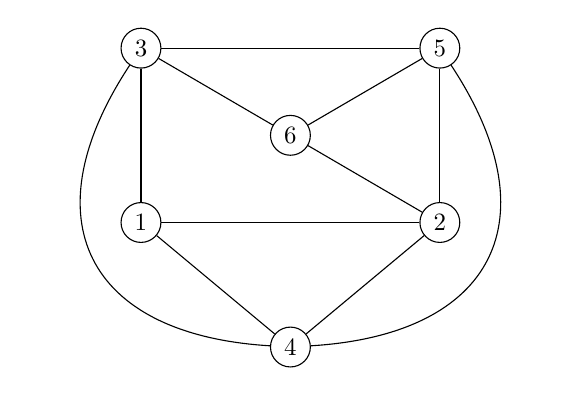
\begin{tikzpicture}[
      x=1pt,y=1pt,
      >=stealth',
      vertex/.style={draw,minimum width=16,minimum height=16,inner sep=0,circle},
      scale = 0.9, transform shape
    ]
    \begin{scope}[every node/.style={vertex}]
      \node (1) at ( 80,75 ) {1};
      \node (2) at (200,75 ) {2};
      \node (3) at ( 80,145) {3};
      \node (4) at (140,25 ) {4};
      \node (5) at (200,145) {5};
      \node (6) at (140,110) {6};
    \end{scope}
    \path
      (1) edge [-]  (2) edge [-] (3) edge [-] (4)
      (2) edge [-] (4) edge [-]  (5) edge [-] (6)
      (3) edge [-,bend right=60,looseness=1.5]  (4) edge [-] (5) edge [-]  (6)
      (4) edge [-,bend right=60,looseness=1.5]  (5)
      (5) edge [-] (6)
      ;
  \end{tikzpicture}
\caption{Undirected graph having 6 nodes and 11 edges}
\label{fig:graph}
\end{figure}

%%% Local Variables:
%%% mode: latex
%%% TeX-master: "paper"
%%% End:

%
\lstinputlisting[float=t,caption={%
ASP facts representing the graph of Figure.~\ref{fig:graph} (\code{graph.lp})},%
captionpos=b,frame=single,label=code:graph.lp,%
numbers=none,%
breaklines=true,%
columns=fullflexible,keepspaces=true,%
basicstyle=\ttfamily\scriptsize]{code_graph_lp.tex}
%
\lstinputlisting[float=t,caption={%
ASP rules for graph coloring (\texttt{color.lp})},%
captionpos=b,frame=single,label=code:color.lp,%
%numbers=none,%
breaklines=true,%
columns=fullflexible,keepspaces=true,%
basicstyle=\ttfamily\scriptsize]{code_color_lp.tex}
%
\lstinputlisting[float=t,caption={Solving a graph coloring problem (\code{graph.lp} and \code{color.lp})},%
captionpos=b,frame=single,label=code:color.log,%
numbers=none,%
breaklines=true,%
columns=fullflexible,keepspaces=true,%
basicstyle=\ttfamily\scriptsize]{code_color_log.tex}
%%%%%%%%%%%%%%%%%%%%%%%%%%%%%%%%%%%%%%%%%

For solving a problem instance of a problem class in ASP, 
we encode the problem instance as a set of ASP facts and the problem
class as a set of ASP rules.
In turn, the facts are combined with the rules, 
and the result is
subsequently solved by an off-the-shelf ASP system that returns
an answer set representing a solution to the original problem.

As an example, let us consider a graph coloring problem.
The problem consists in finding
assignments of colors to nodes such that no two nodes connected by an
edge have the same color. 
A problem instance is given by a graph as in Figure~\ref{fig:graph}.
%
It is represented as facts of predicates
\code{node/1} and \code{edge/2} in Listing~\ref{code:graph.lp}.
The 3-colorability problem class is encoded in Listing~\ref{code:color.lp}.
%
Line 1 provides the available colors as facts.
Line 3 and 4 express the actual colorability problem.
The predicate \code{color(X,C)} is used to express that a node
\code{X} is colored with \code{C}.
%
The rule in Line 3 generates for each node \code{X} a set of candidate assignments
subject to the condition that there is exactly one color \code{C} such that \code{color(X,C)} holds.
In detail, the conditional literal
\code{color(X,C):col(C)}
in the cardinality constraint
expands to the conjunction of 
\code{color(X,r)}, \code{color(X,b)}, and \code{color(X,g)}, since
the facts \code{col(r)}, \code{col(b)}, and \code{col(g)} unconditionally hold.
That is, line 3 expresses that each node \code{X} must be colored with
exactly one color among red (\code{r}), blue (\code{b}), and green (\code{g}).
%
The integrity constraint in Line 4 expresses that all connected nodes
\code{X} and \code{Y} must not be colored with the same color \code{C},
since, as mentioned above, 
the conjunction of literals in its body must not hold. 
%
Line 6 is a directive, that is, a meta statement advising the ASP system to project answer sets
onto instances of predicate \code{color/2}.
%
An answer set computed by the ASP system {\clingo} is shown in
Listing~\ref{code:color.log}; 
it represents a coloring of node \code{1} with green,
\code{2} and \code{3} with blue, 
\code{4} with red, 
\code{5} with green, and 
\code{6} with red.

Modern ASP systems like {\clingo} first translate
user-defined logic programs (with variables) into 
equivalent ground (that is, variable-free) programs, 
and then compute the answer sets of the ground programs.
Particularly, the former task is called \emph{grounding}.
The foundations and algorithms underlying the technology of {\clingo}
are described in detail in \citep{gekakasc12a}.

%%% Local Variables:
%%% mode: latex
%%% TeX-master: "paper"
%%% End:

\section{The {\asap} Approach}\label{sec:approach}

We begin with describing {\asap}'s fact format of CB-CTT instances and
then present a basic {\asap} encoding for solving the CB-CTT problems
\footnote{{\asap}: \textbf{T}im\textbf{E}tabling with \textbf{A}nswer \textbf{S}et \textbf{P}r\textbf{O}grammi\textbf{N}g}.
%%%%%%%%%%%%%%%%%%%%%%%%%
\subsection{Fact Format}
%\textbf{Fact Format.}
%%%%%%%%%%%%%%%%%%%%%%%%%
\begin{figure}[t]
\centering
\begin{minipage}[t]{.45\textwidth}
\lstinputlisting[caption={A toy instance of the \code{ectt} format},%
captionpos=b,frame=single,label=ex:toy.ectt,%
numbers=none,%
basicstyle=\ttfamily\scriptsize]{code_toy1_ectt.tex}
\end{minipage}\hfill
\begin{minipage}[t]{.45\textwidth}
\lstinputlisting[frame=single,numbers=none,%
basicstyle=\ttfamily\scriptsize]{code_toy2_ectt.tex}
\end{minipage}
\end{figure}
%
\lstinputlisting[float=t,caption={ASP facts representing the toy instance of Listing~\ref{ex:toy.ectt}},%
captionpos=b,frame=single,label=ex:toy.lp,%
%numbers=none,%
breaklines=true,%
columns=fullflexible,keepspaces=true,%
basicstyle=\ttfamily\scriptsize]{code_toy_lp.tex}
%
\lstinputlisting[float=t,caption={Solution (partial answer set) of the toy instance in UD2},%
captionpos=b,frame=single,label=ex:toy_out.lp,%
%numbers=none,%
breaklines=true,%
columns=fullflexible,keepspaces=true,%
basicstyle=\ttfamily\scriptsize]{code_toy_sol_lp.tex}
%%%%%%%%%%%%%%%%%%%%%%%%%
Listing~\ref{ex:toy.ectt} shows a toy instance of the \code{ectt}
format, which is a standard input format of CB-CTT 
instances~\citep{DBLP:journals/anor/BonuttiCGS12}.
The format has headers that represent basic entities, followed
by five blocks, 
\code{COURSES}, 
\code{ROOMS}, 
\code{CURRICULA}, 
\code{UNAVAILABILITY_CONSTRAINTS}, and 
\code{ROOM_CONSTRAINTS}.

ASP facts representing the toy instance are shown in
Listing~\ref{ex:toy.lp}.
There exists a one-to-one correspondence between ASP fact format and
the \code{ectt} format except for the \code{CURRICULA} block.
%
The facts in Line 1--2 correspond to the \code{ectt} headers and
express that
the instance named \texttt{Toy} consists of 
4 courses, 
3 rooms,
2 curricula,
8 unavailability constraints, and 
3 room constraints.
The weekly timetable consists of 
5 days and 4 periods per day, which start from 0.
The fact \code{min_max_daily_lectures(2,3)} expresses 
the minimum and maximum numbers of daily lectures 
for each curriculum, and is used to specify $S_6$.

Each fact of predicate \code{course/6} in Line 4--5
corresponds to a line of the \code{COURSES} block.
A fact \texttt{course($C$,$T$,$N$,$MWD$,$M$,$DL$)}
expresses that a course $C$ taught by a teacher $T$ 
consists of $N$ lectures, which must be spread into $MWD$ days.  
The number of students attending the course $C$ is $M$.  
The course $C$ requires double lectures if $DL=1$.  
%
Each fact of predicate \code{room/3} in Line 7 
corresponds to a line of the \code{ROOMS} block.
A fact \texttt{room($R$,$CAP$,$BLD$)} expresses that a
room $R$ in a building $BLD$ has a seating capacity of $CAP$.

A fact \texttt{curricula($CUR$, $C$)} in Line 9--10 expresses that
a course $C$ belongs to a curriculum $CUR$.
%
Each fact of predicate \code{unavailability_constraint/3} in Line
12--15 corresponds to a line of the 
\code{UNAVAILABILITY_CONSTRAINTS} block, and is used to specify $H_4$.
A fact \texttt{unavailability\_constraint($C$,$D$,$P$)}
expresses that a course $C$ is not available at a period $P$ on a day
$D$.
%
Each fact of predicate \code{room_constraint/2} in Line 17
corresponds to a line of the \code{ROOM_CONSTRAINTS} block, and
is used to specify $S_8$.
A fact \texttt{room\_constraint($C$,$R$)} expresses that a room $R$ is
not suitable for a course $C$.

Listing~\ref{ex:toy_out.lp} shows an optimal solution with zero penalty
of the toy instance in the UD2 formulation.
Each atom \texttt{assigned($C$,$R$,$D$,$P$)} is intended to
express that a lecture of a course $C$ is assigned to 
a room $R$ at a period $P$ on a day $D$.
We can observe from Line 1 that
the lectures of the course \texttt{SceCosC} are
assigned to the room \texttt{rB} at
the first period (\texttt{0}) on Thursday (\texttt{3}),
the third period (\texttt{2}) on Wednesday (\texttt{2}), and
the third period (\texttt{2}) on Friday (\texttt{4})


\subsection{First-Order Encoding}
%\textbf{First-Order Encoding.}
%%%%%%%%%%%%%%%%%%%%%%%%%
\lstinputlisting[float=t,caption={Encoding of hard constraints},%
captionpos=b,frame=single,label=en:ctt_hard2.lp4,%
%numbers=none,%
breaklines=true,%
columns=fullflexible,keepspaces=true,%
basicstyle=\ttfamily\scriptsize]{code_hard_lp.tex}
%%%%%%%%%%%%%%%%%%%%%%%%%
\lstinputlisting[float=t,caption={Encoding of soft constraints and objective function},%
captionpos=b,frame=single,label=en:ctt_soft.lp4,%
%numbers=none,%
breaklines=true,%
columns=fullflexible,keepspaces=true,%
basicstyle=\ttfamily\scriptsize]{code_soft_lp.tex}
%%%%%%%%%%%%%%%%%%%%%%%%%
The {\asap} encoding of hard constraints ($H_1$--$H_4$) is shown in 
Listing~\ref{en:ctt_hard2.lp4}.
The expressive power of ASP's modelling language enables us to express
each hard constraint individually by just one or two ASP rules.
%
As mentioned, the atom \texttt{assigned($C$,$R$,$D$,$P$)}
expresses that a lecture of a course $C$ is assigned to a room $R$ at
a period $P$ on a day $D$, and a solution is composed of 
a set of these assignments.
The atom \texttt{assigned($C$,$D$,$P$)} dropping $R$
from \texttt{assigned($C$,$R$,$D$,$P$)} is also introduced,
since we do not always have to take the room information into account 
to specify the hard constraints except $H_3$.

Given an instance expressed in our fact format,
the first four rules in Line 1--2 generate 
\code{c(C)}, 
\code{t(T)}, 
\code{r(R)}, and
\code{cu(Cu)} 
for each course \code{C}, teacher \code{T}, room \code{R}, and 
curriculum \code{Cu}.
%
The next two rules in Line 3 generate 
\code{d(0)} $\ldots$ \code{d(D-1)} and
\code{ppd(0)} $\ldots$ \code{ppd(P-1)} 
expressing that the days range from \code{0} to \code{D-1}, 
and the periods per day range from \code{0} to \code{P-1}.

For $H_1$,
the rule in Line 6,
for every course \code{C} having \code{N} lectures,
generates a set of candidate assignments
subject to the condition that 
there are exactly \code{N} lectures such that \code{assigned(C,D,P)} holds.

For $H_2$,
the rule in Line 9 enforces that,
for every teacher \code{T}, day \code{D}, and period \code{P},
there is at most one course \code{C} taught by \code{T}
such that \code{assigned(C,D,P)} holds.
In detail, 
if \code{t(T)}, \code{d(D)}, and \code{ppd(P)} hold,
this integrity constraint tells us that
the at-most-one constraint represented by 
`\verb+{ assigned(C,D,P) : course(C,T,_,_,_,_) } 1+'
must be true as well in order to prevent its body from being satisfied. 
In the similar way,
the rule in Line 10 enforces that,
for every curriculum \code{Cu}, day \code{D}, and period \code{P},
there is at most one course \code{C} that belongs to \code{Cu}
such that \code{assigned(C,D,P)} holds.

For $H_3$, 
if \code{assigned(C,D,P)} holds, 
the rule in Line 13 generates a solution candidate 
subject to the condition that there is exactly one room \code{R} such
that \code{assigned(C,R,D,P)} holds. 
The rule in Line 14 enforces that,
for every room \code{R}, day \code{D}, and period \code{P},
there is at most one course \code{C} such that 
\code{assigned(C,R,D,P)} holds.

For $H_4$,
the rule in Line 17 enforces that
a course \code{C} is not assigned at a period \code{P} on a day \code{D}
if \code{unavailability_constraint(C,D,P)} holds, since
the conjunction of literals in its body must not hold. 

The rule in Line 20 expresses that 
for each timeslot (\code{D} and \code{P})
the number of lectures assigned must be less than or equal to 
the number of rooms (\code{N}).
This rule is an implied constraint and can be omitted, but we keep it
as an additional rule for performance improvement of some problem
instances.

The {\asap} encoding of soft constraints ($S_1$--$S_9$) and an
objective function is shown in Listing~\ref{en:ctt_soft.lp4}.
We introduce a \textit{penalty atom}
\texttt{penalty($S_i$,$V$,$C$)}, which is intended to express
that a constraint $S_i$ is violated by $V$ and its penalty cost is $C$.
The constants denoted by \code{weight_of_*} indicate
the weights associated with each soft constraint defined in
Table~\ref{table:problem_formulations}.
%
Once again, each soft constraint $S_i$ is compactly expressed by
just one or two ASP rules in which the head is of the form
\texttt{penalty($S_i$,$V$,$C$)}, and a violation $V$ and its penalty
cost $C$ are detected and calculated respectively in the body.
That is, for each violation $V$ of $S_i$, 
an atom \texttt{penalty($S_i$,$V$,$C$)} is generated.
Optimal solutions can be obtained by
minimizing the number of penalty atoms in Line 49.

We explain $S_{1}$--$S_{3}$ that compose the basic UD1 formulation.
%
For $S_1$, 
the rule in Line 2--3,
for every course \code{C} that \code{N} students attend and
room \code{R} that has a seating capacity of \code{Cap},
generates a penalty atom with the cost of 
\code{(N-Cap)*weight_of_s1}
if a lecture of course \code{C} is assigned to the room \code{R}
whose seating capacity (\code{Cap}) is less than the number of
attendees (\code{N}).

For $S_2$,
the rule in Line 6 generates an auxiliary atom \code{working_day(C,D)}
which expresses that a course \code{C} is given on a day \code{D}, 
if \code{assigned(C,D,P)} holds.
The rule in Line 7--8,
for every course \code{C} whose lectures 
must be spread into \code{MWD} days,
generates a penalty atom with the cost of 
\code{(MWD-N)*weight_of_s2},
if the number of days (\code{N}) in which a course \code{C} spread
is less than \code{MWD}.

For $S_3$, 
the rule in Line 11 generates an auxiliary atom \code{scheduled_curricula(Cu,D,P)}
which expresses that 
a curriculum \code{Cu} is 
scheduled at a period \code{P} on a day \code{D},
if \code{assigned(C,D,P)} holds.
% Note that, by $H_2$,
% for every curriculum \code{Cu}, day \code{D}, and period \code{P},
% there must be at most one course \code{C} that belongs to \code{Cu}
% such that \code{assigned(C,D,P)} holds. 
The rule in Line 12--14,
for every curriculum \code{Cu}, day \code{D}, and period \code{P},
generates a penalty atom with the cost of \code{weight_of_s3},
if a curriculum \code{Cu} is scheduled at a period \code{P} on a
day \code{D}, but not at both \code{P-1} and \code{P+1} 
within the same day \code{D}.


%%% Local Variables:
%%% mode: latex
%%% TeX-master: "paper"
%%% End:

\section{Extensions}\label{sec:ext}

We here extend the basic {\asap} encoding presented in
Section~\ref{sec:approach} in view of enhancing the scalability and
flexibility of solving (multi-criteria) CB-CTT problems.
For scalability, we describe a collection of optimized {\asap}
encodings for soft constraints in Section~\ref{subsec:ext:soft}.
For flexibility, we present significant extensions for 
easy composition of different
formulations in Section~\ref{subsec:ext:formulations} as well as for
multi-criteria optimization based on lexicographic ordering in
Section~\ref{subsec:ext:lex}.
And finally, 
we discuss the possibility of multi-shot ASP solving with
{\asap} and illustrate a neighborhood search using (a part of) legacy
timetables in Section~\ref{subsec:ext:multishot}.

\subsection{Optimized encodings for soft constraints}
\label{subsec:ext:soft}
%%%%%%%%%%%%%%%%%%%%%%%%%
\lstinputlisting[float=t,caption={A collection of optimized encodings for $S_2$, $S_4$, $S_6$, and $S_7$},%
captionpos=b,frame=single,label=en:roland_soft.lp4,%
%numbers=none,%
breaklines=true,%
columns=fullflexible,keepspaces=true,%
basicstyle=\ttfamily\scriptsize]{code_roland_soft_lp.tex}
%%%%%%%%%%%%%%%%%%%%%%%%%

The basic encoding in Section~\ref{sec:approach} precisely reflects
the definition of CB-CTT constraints, 
but fails to scale to large instances in complex formulations like
UD5 due to expensive grounding.
To solve this practical issue, we present optimized encodings for the soft constraints
$S_2$.~MinWorkingDays, 
$S_4$.~Windows, 
$S_6$.~StudentMinMaxLoad, and 
$S_7$.~TravelDistance.

%
For $S_7$,
the rule in Line 35--37 of Listing~\ref{en:ctt_soft.lp4}
generates a penalty atom with the constant cost of \code{weight_of_s7}
if both
\code{assigned(C1,R1,D,P)} and \code{assigned(C2,R2,D,P+1)} hold 
for 
two courses \code{C1} and \code{C2} that belong to the same curriculum \code{Cu}, 
day \code{D}, and period \code{P},
and
rooms \code{R1} and \code{R2} located in different buildings.
This rule is very expensive when grounding due to its combinatorial blow-up
caused by many variables.
This issue can be improved by taking into account that
for every curriculum \code{Cu}, room \code{R}, day \code{D}, and period \code{P},
there is at most one course \code{C} that belongs to \code{Cu}
such that \code{assigned(C,R,D,P)} holds. 

In view of this,
an optimized encoding of $S_7$ is shown in Line 2--4 of
Listing~\ref{en:roland_soft.lp4}.
The difference from the basic one is that a new predicate
\code{scheduled_curricula/4} is introduced.
The atom \code{scheduled_curricula(Cu,B,D,P)} is intended to express that 
a curriculum \code{Cu} is scheduled in a building \code{B} at a period
\code{P} on a day \code{D}.
The rule in Line 2
generates an atom \code{scheduled_curricula(Cu,B,D,P)} if \code{assigned(C,R,D,P)} holds
for every curriculum \code{Cu}, course \code{C} that belongs to
\code{Cu}, room \code{R} located in a building \code{B}, day \code{D}, and period \code{P}.
%
The rule in Line 3--4
produces a penalty atom with the constant cost of \code{weight_of_s7}
for every curriculum \code{Cu}, day \code{D}, and period \code{P},
if a curriculum \code{Cu} is scheduled in different buildings at
period \code{P} and \code{P+1} within the same day \code{D}.
%
Another optimized encoding of $S_7$ is shown in Line~7--9 of
Listing~\ref{en:roland_soft.lp4}.
The difference from the other two is that it utilizes cardinality constraints for 
counting the number of buildings which are used by 
two lectures belonging the same curriculum
in two adjacent periods within the same day.

An optimized encoding of $S_4$ is shown in Line 12--19 of
Listing~\ref{en:roland_soft.lp4}.
The newly introduced atom \code{scheduled_curricula_chain(Cu,D,P,DP)} 
is intended to express that 
there is a course in curriculum \code{Cu} scheduled before a period
\code{P} in a day \code{D} if \code{DP = -1}, or else if \code{DP = 1}
the course in \code{Cu} is scheduled after \code{P}.
The rule in Line 16--19
generates a penalty atom with the constant cost of \code{weight_of_s4}
for every curriculum \code{Cu}, day \code{D}, and period \code{P},
if there is a time window \code{P} for \code{Cu} in a day \code{D}.

In the basic encoding, the soft constraints $S_2$ and $S_6$ are
expressed by using ASP's cardinality constraints.
These rules can be optimized by using state-of-the-art SAT encoding
techniques for Boolean cardinality constraints.
We used Sinz's sequential counter encoding~\citep{sinz05a},
and the resulting encodings are shown in 
Line 22--27 for $S_2$ and Line 30--45 for $S_6$.
For $S_2$,
the atom \texttt{wd\_counter($C$,$M$,$D$,$N$)}
is intended to express that 
the number of lectures scheduled from day 0 to $D$ for a course $C$
whose lectures must be spread into $M$ days is greater than or equal to $N$.
The rule in Line 26--27
generates a penalty atom with the constant cost of \code{weight_of_s2}
for every course \code{C} whose lectures must be spread into \code{M} days,
if the number of lectures for \code{C} scheduled in the whole days is
less than \code{M}.
The basic rules of $S_6$ is optimized in a similar way.

\subsection{Easy composition of different formulations}
\label{subsec:ext:formulations}
%%%%%%%%%%%%%%%%%%%%%%%%%
\lstinputlisting[float=t,caption={Extended encoding of $S_8$ and $H_4$},%
captionpos=b,frame=single,label=en:ctt_ext_room_suitability.lp,%
%numbers=none,%
breaklines=true,%
columns=fullflexible,keepspaces=true,%
basicstyle=\ttfamily\scriptsize]{code_s8_h4_lp.tex}
%
\lstinputlisting[float=t,caption={The UD4 formulation},%
captionpos=b,frame=single,label=en:ctt_ext_ud4.lp4,%
numbers=none,%
basicstyle=\ttfamily\scriptsize]{code_ud4_lp.tex}
%
\lstinputlisting[float=t,caption={Formulation consisting of %
all soft constraints ($S_1$--$S_9$) with the weights of all 1s},%
captionpos=b,frame=single,label=en:ctt_ext_ud0.lp4,%
numbers=none,%
basicstyle=\ttfamily\scriptsize]{code_udall_soft_lp.tex}
%%%%%%%%%%%%%%%%%%%%%%%%%

Problem modeling is particularly challenging in the real-world
course timetabling, since 
different institutions have their own needs and policies, and
formulations (sets of constraints) may change from institution to
institution and from time to time~\citep{DBLP:conf/patat/McCollum06}.
In this view, we present a design for easy composition of different
formulations.

In order to easily activate or deactivate each soft constraint and
switch it from soft to hard, we introduce new predicates 
\code{soft_constraint/3} and
\code{hard_constraint/1}.
The atom \texttt{soft\_constraint($S_i$,$W_i$,$L_i$)} is intended to
express that $S_i$ is a soft constraint to be activated.
$W_i$ and $L_i$ respectively represent the weight and the priority
level associated with $S_i$.
The priority level $L_i$ is used for lexicographic optimization explained later.
%
The atom \texttt{hard\_constraint($S_i$)} is intended to express that
$S_i$ is activated as a hard constraint.
We refer to these atoms as \textit{constraint atoms}.

Listing~\ref{en:ctt_ext_room_suitability.lp} shows
extended encodings of 
$S_8$.RoomSuitability and 
$H_4$.Availability with constraint atoms.
For $S_8$, the rule in Line 2--3 is the same as before
except that an instance of \code{soft_constraint/3} is added.
Note that the penalty atom in its head is extended to
\code{penalty/4} with a priority level $L_i$.
The integrity constraint in Line 6 expresses $S_8$ as a hard
constraint by dropping the penalty atom in the head in Line 2--3.
%
% Alternatively, 
% switching from soft to hard can be done by enforcing a
% cardinality constraint like 
% `\lstinline|:- not #sum { P,C,L : penalty("RoomSuitability",C,P,L) } 0.|'.
% In this case, we don't need 
% the rule in Line 6 that expresses $S_8$ as a hard constraint.
On the other hand,
it is also possible to switch constraints in the opposite direction,
that is, from hard to soft.
For example, to define $H_4$ as a soft constraint, we only have to add
a penalty atom to the head of the rule in Line 17 of
Listing~\ref{en:ctt_hard2.lp4}.
An extended encoding of $H_4$ with constraint atoms is shown in 
Line 8--14 of Listing~\ref{en:ctt_ext_room_suitability.lp}.
The other constraints can be extended in a similar way.

The idea of constraint atoms allows for easy composition of different
formulations, since any combination of constraints can be represented
as a set of ASP facts. 
Consequently, it enables a timetable keeper to experiment with
different formulations at a purely declarative level.
For example, ASP facts representing the UD4 formulation
are shown in Listing~\ref{en:ctt_ext_ud4.lp4}.
And also, we show exhaustive formulation consisting of all soft constraints
($S_1$--$S_9$) with the weights of all set to 1 
in Listing~\ref{en:ctt_ext_ud0.lp4}\footnote{%
Surprisingly, the {\asap} system was able to find an optimal %
solution of \code{comp11} in this formulation.}.
These two examples represent single-objective weighted-sum
formulations, since the priority levels are all 0.

\subsection{Multi-criteria optimization based on lexicographic ordering}
\label{subsec:ext:lex}
%%%%%%%%%%%%%%%%%%%%%%%%%
\lstinputlisting[float=t,caption={Objective function with priority levels for lexicographic optimization},%
captionpos=b,frame=single,label=en:ctt_minimize_mo.lp4,%
numbers=none,%
basicstyle=\ttfamily\scriptsize]{code_obj_lp.tex}
%
\lstinputlisting[float=t,caption={The UD5 formulation with different priority levels},%
captionpos=b,frame=single,label=en:ud5_lex.lp,%
numbers=none,%
basicstyle=\ttfamily\scriptsize]{code_ud5_lex_lp.tex}
%%%%%%%%%%%%%%%%%%%%%%%%%
A well-known multi-criteria optimization strategy called lexicographic
ordering~\citep{Marler2004} has been implemented in {\clingo}. 
It enables us to optimize criteria in a lexicographic order based on
their priorities.
We here extend the {\asap} encoding for supporting such multi-criteria optimization.

This extension can be done by adding priority levels to the \code{#minimize}
function, as can be seen in Listing~\ref{en:ctt_minimize_mo.lp4}.
The variable \code{L} on the right-hand side of \code{@} stands for 
a priority level, where greater levels are more significant than
smaller ones.
Usually, solutions can be represented in the form of a utility vector
$(p_1,p_2,\dots,p_n)$, where each $p_i$ is a value 
representing the penalty of a soft constraint.

Such lexicographic optimization is quite useful, since 
it enables a timetable keeper to experiment with different
(pre-defined) priority levels of soft constraints.
%
On the other hand,
the optimality of multi-criteria optimization 
with lexicographic ordering does not always
coincide with that of single-objective 
weighted-sum one.
However, 
optimal solutions 
as well as better vectors
obtained by lexicographic optimization
can often correspond to feasible ones with smaller penalty
in the original single-objective setting.

For illustration, Listing~\ref{en:ud5_lex.lp} shows an UD5 formulation
with lexicographic optimization in which 
the priority levels of soft constraints are ordered as 
$S_1 > S_4 > S_2 > S_7 > S_6 > S_3$.
In this case, the optimal solution of 
the ITC-2007 instance \code{comp13}
is $(S_1,S_4,S_2,S_7,S_6,S_3) = (0,0,0,0,112,35)$.
This optimum corresponds to a smaller bound
$112+35=147$ than the best known one 
in the CB-CTT portal 
obtained by single-objective weighted-sum optimization.
A more detailed analysis of lexicographic optimization is shown in 
Section~\ref{subsec:eval:ext}.

%%%%%%%%%%%%%%%%%%%%%%%%%%%%%%%%%%%%%%%%%%%%%%%%%%%%%%%%%%%%%%%%%%%%%%%%%
\subsection{Discussion towards multi-shot ASP solving with {\asap}}
\label{subsec:ext:multishot}

Suppose that a (part of) legacy timetable is represented as a set of
ASP facts of predicate \code{legacy/1}.
ASP-based neighborhood search is implemented by only one rule:
%%%%%%%%%%%%%%%%%%%%%%%%%
\lstinputlisting[numbers=none,basicstyle=\ttfamily\small]{code_heu_lp.tex}
%%%%%%%%%%%%%%%%%%%%%%%%%
The special statement \code{#heuristic} is used to express
various modifications to {\clingo}'s heuristic treatment of atoms.
This rule
expresses a preference for both making a decision on 
\code{assigned(C,R,D,P)} and assigning it to true if 
\code{legacy(assigned(C,R,D,P))} holds
for every course \code{C}, room \code{R}, day \code{D}, and period \code{P}.

Incremental SAT solving has recently been recognized as an important
technique for many problems such as model checking and
planning~\citep{DBLP:journals/entcs/EenS03}.
From an ASP perspective,
such multi-shot ASP solving is also available in {\clingo}~\citep{gekaobsc15a}.
It enables us to handle problem specifications which evolve during the
reasoning process,  because either data or constraints are added,
deleted, or replaced.

For (multi-criteria) CB-CTT solving, multi-shot ASP solving with
\asap\ can be promising.
This is because it provides an incremental solving framework
for finding optimal
solutions as well as better bounds, 
while varying a set of constraints, 
switching them from hard to soft, 
varying the priority level of objectives, and 
searching neighborhoods by using a (part of) legacy timetables.

%%% Local Variables:
%%% mode: latex
%%% TeX-master: "paper"
%%% End:


\section{Propagator Interface}\label{sec:system}

We now turn to the implementation of theory propagation in \clingo~5
and detail the structure of its interface depicted in Figure~\ref{fig:interface}.
%
\begin{figure}
  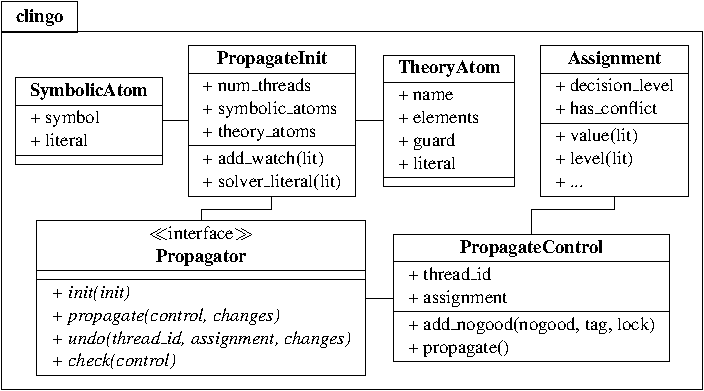
\includegraphics[width=\textwidth]{figures/python-interface}
  \caption{Class diagram of \clingo's (theory) propagator interface\label{fig:interface}}
\end{figure}
%
% To begin with,
The interface \code{Propagator} has to be implemented by each custom propagator.
After registering such a propagator with \clingo,
its functions are called during initialization and search as indicated % in the algorithm
in Figure~\ref{fig:cdcl}.
%
Function \code{Propagator.init}%
\footnote{For brevity, we below drop the qualification \code{Propagator} and use its function names unqualified.}
is called once before solving (Line~(\ref{fig:cdcl:init}) in Figure~\ref{fig:cdcl})
to allow for initializing data structures used during theory propagation.
It is invoked with a \code{PropagateInit} object providing access to symbolic (\code{SymbolicAtom}) as well as theory (\code{TheoryAtom}) atoms.
Both kinds of atoms are associated with program literals,\footnote{Program literals are also used in the \aspif\ format (see~\ref{sec:aspif}).} % ~\cite{gekakaosscwa16b}
which are in turn associated with solver literals.%
\footnote{Note that \clasp's preprocessor might associate a positive or even negative solver literal with multiple atoms.}
Program as well as solver literals are identified by non-zero integers, where positive and negative numbers represent positive or  negative literals, respectively.
In order to get notified about assignment changes, a propagator can set up watches on solver literals during initialization.

During search, function \codeClass{Propagator}{propagate} is called with a \code{PropagateControl} object
and a (non-empty) list of watched literals that got assigned in the recent round of unit propagation (Line~(\ref{fig:cdcl:propagate}) in Figure~\ref{fig:cdcl}).
The \code{PropagateControl} object can be used to inspect the current assignment, record nogoods, and trigger unit propagation.
Furthermore, to support multi-threaded solving,
its \code{thread\_id} property identifies the currently active thread,
each of which can be viewed as an independent instance of the CDCL algorithm in Figure~\ref{fig:cdcl}.%
%Hence, thread-specific state has to be associated with the \code{thread\_id}.
\footnote{%
Depending on the configuration of \clasp, threads can communicate with each other.
For example, some of the recorded nogoods can be shared.
This is transparent from the perspective of theory propagators.}
%
Function \codeClass{Propagator}{undo} is the counterpart of \codeClass{Propagator}{propagate}
and called whenever the solver retracts assignments to watched literals (Line~(\ref{fig:cdcl:undo}) in Figure~\ref{fig:cdcl}).
In addition to the list of watched literals that have been retracted (in chronological order),
it receives the identifier and the assignment of the active thread.
%
Finally, function \codeClass{Propagator}{check} is similar to \codeClass{Propagator}{propagate},
yet invoked without a list of changes.
Instead, it is (only) called on total assignments
(Line~(\ref{fig:cdcl:check}) in Figure~\ref{fig:cdcl}), independently of watches.
%
Overriding the empty default implementations of propagator methods is optional.
% Implementing the propagator methods, which default to empty implementations, is optional. % that does nothing.
For brevity, we below focus on implementations of the methods in \python,
while \lua\ or \C\ could be used as well.

For illustration,
consider Listing~\ref{prg:pigeon:propagator} giving a propagator for (half of) the pigeon-hole problem.
%
\lstinputlisting[linerange={1-10,12-39},float=t,mathescape=true,escapeinside={\#(}{\#)},basicstyle={\ttfamily\small},label={prg:pigeon:propagator},caption={Propagator for the pigeon-hole problem},language=clingo]{example/pigeon-py.lp}
%
Although this setting is constructed, it showcases central aspects
that are also relevant when implementing more complex propagators,
e.g., the \code{Pigeonator} is both stateful and can be used with multiple threads.
%
The underlying ASP encoding is given in Line~\ref{prg:pigeon:prop:rule1}:
A (choice) rule generates solution candidates by placing each of the $p$ pigeons in exactly one among $h$ holes.
While the rule commented out in Line~\ref{prg:pigeon:prop:rule2} would ensure that there is at most one pigeon per hole,
this constraint is handled by the \code{Pigeonator} class
implementing the \code{Propagator} interface (except for \code{check}) in Lines~\ref{prg:pigeon:prop:begin-init}--\ref{prg:pigeon:prop:end-undo}.
Whenever two pigeons are placed in the same hole, it adds a binary nogood forbidding the placement.
To this end,
it maintains data structures for, given a newly placed pigeon,
detecting whether there is a conflict.
%
More precisely, the propagator has two data members:
The \code{self.place} dictionary in Line~\ref{prg:pigeon:prop:member-place} maps solver literals
for \code{place}$/2$ atoms to their corresponding holes,
and the \code{self.state} list in Line~\ref{prg:pigeon:prop:member-state} stores for each solver thread its current placement of pigeons
as a mapping from holes to true solver literals for \code{place}$/2$ atoms.

Function \codeClass{Pigeonator}{init} in Lines~\ref{prg:pigeon:prop:begin-init}--\ref{prg:pigeon:prop:end-init}
sets up watches as well as the dictionaries in \code{self.place} and \code{self.state}.
%
To this end,
it traverses (symbolic) atoms over \code{place}$/2$ in Lines~\ref{prg:pigeon:prop:init:loop-atoms}--\ref{prg:pigeon:prop:init:end-loop-atoms}.
Each such atom is associated with a solver literal, % in \clasp,
obtained in Line~\ref{prg:pigeon:prop:init:map-literal}.
The mapping from the solver literal to its corresponding hole is then stored in the \code{self.place} dictionary in
Line~\ref{prg:pigeon:prop:init:map-lit-hole}.
%
In the last line of the loop, a watch is added for each solver literal at hand,
so that the solver calls \code{propagate} whenever a pigeon is placed. % in the hole as specified by the placement atom.
%
Finally, in Line~\ref{prg:pigeon:prop:init:state}, the \code{self.state} list
of placements per thread,
subject to change upon propagation and backjumping,
% Given a solving thread $i$, each state \code{self.state[$i$]} is a dictionary mapping holes to placement atoms given by their literals.
is initialized with empty dictionaries.

Function \codeClass{Pigeonator}{propagate}, given in Lines~\ref{prg:pigeon:prop:begin-prop}--\ref{prg:pigeon:prop:end-prop},
accesses \code{control.thread\_id} in Line~\ref{prg:pigeon:prop:prop:state}
to obtain the \code{holes} dictionary storing the active thread's current placement of pigeons.
% At first, in Line~\ref{prg:pigeon:prop:prop:state},
% \code{control.thread\_id} is used to obtain the dictionary storing the current thread's partial placement of pigeons.
The loop in Lines~\ref{prg:pigeon:prop:prop:begin-loop}--\ref{prg:pigeon:prop:prop:end-loop} then iterates over the list of changes,
i.e., solver literals representing newly placed pigeons.
After in Line~\ref{prg:pigeon:prop:prop:pigeon-to-hole}
determining the \code{hole} associated with a recently assigned literal,
% , the target \code{hole} associated with the current literal is obtained.
% Then,
\python's \code{setdefault} function is used to update the state:
Depending on whether \code{hole} already appears as a key in the \code{holes} dictionary,
the function either retrieves its associated literal or inserts the new literal under key \code{hole}. % into the dictionary.
While the latter case amounts to updating the placement of pigeons, the former signals a conflict,
triggered by recording a binary nogood in Line~\ref{prg:pigeon:prop:prop:add-clause}.
% In case of a conflict, the propagator adds a binary nogood in Line~\ref{prg:pigeon:prop:prop:add-clause} preventing such an invalid placement of pigeons.
Given that the solver has to resolve the conflict and backjump,
the call to \code{add\_nogood} always yields false, so that
propagation stops without processing remaining changes any further.\footnote{%
  The optional arguments \code{tag} and \code{lock} of \code{add\_nogood} can be used to control the scope and lifetime of recorded nogoods.
  Furthermore, in a propagator that does not add violated nogoods only, % but also unit-resulting nogoods
  function \code{control.propagate} can be invoked to trigger unit propagation.
  }
% Furthermore, using dictionaries \code{state[i]} and \code{place}, conflicts are detected in constant time.

Function \codeClass{Pigeonator}{undo} in Lines~\ref{prg:pigeon:prop:begin-undo}--\ref{prg:pigeon:prop:end-undo} resets a thread's placement of pigeons upon backjumping.
Similar to \codeClass{Pigeonator}{propagate}, % it is called by each solving thread.
the active thread's current placement
is obtained in Line~\ref{prg:pigeon:prop:undo:state},
and changes are traversed in Lines~\ref{prg:pigeon:prop:undo:begin-loop}--\ref{prg:pigeon:prop:undo:del}.
% The function then loops over the set of changes,
% that is, the literals corresponding to pigeons to be removed from the partial placement in Line~\ref{prg:pigeon:prop:undo:del}.
The latter correspond to retracted solver literals,
for which the condition in Line~\ref{prg:pigeon:prop:undo:test} makes sure
that exactly those stored in Line~\ref{prg:pigeon:prop:prop:setdefault} before are cleared,
thus reflecting that the \code{hole} determined in Line~\ref{prg:pigeon:prop:undo:pigeon-to-hole}
is free again.
%%
Finally,
function \code{main} in Lines~\ref{prg:pigeon:prop:begin-main}--\ref{prg:pigeon:prop:end-main} first registers the \code{Pigeonator} propagator in Line~\ref{prg:pigeon:prop:register},
and then initiates grounding and solving with \clingo.

%%% Local Variables:
%%% mode: latex
%%% TeX-master: "paper"
%%% End:

\section{Multi-objective Course Timetabling considering Minimal Perturbation Problems}\label{mpp}

%%%%%%%%%%%%%%%%%%%%%%%%%
\lstinputlisting[float=t,caption={ASP Encoding of the Manhattan distance},%
captionpos=b,frame=single,label=en:distance.lp,%
numbers=none,%
basicstyle=\ttfamily\scriptsize]{code_distance_lp.tex}
%%%%%%%%%%%%%%%%%%%%%%%%%

\emph{The Multi-Objective Discrete Optimization Problem} (MODOP; \citep{Ehrgott2005})
is a problem involving multiple objective functions 
that should be considered separately and optimized simultaneously. 
It is therefore well suited for modeling many real world 
applications involving multiple criteria, such as 
decision making,  %\cite{BB17791648,figueira2005multiple}, 
scheduling,  %\cite{DBLP:journals/anor/BurkeLQ12,DBLP:journals/itor/IturriagaDN17}, 
automated planning,  %\cite{AlarconRodriguez20101353,DBLP:conf/ijcai/YiGS15}, 
%product design %\cite{DBLP:books/daglib/0027803}
etc.
%
The goal of this problem is finding the \emph{Pareto front}
(viz. the set of Pareto optimal solutions) 
defined by Pareto optimality.
Usually, a Pareto optimal solution is expressed in the form of
utility vector $(o_1,o_2,\ldots, o_n)$
where each $o_i$ is a value representing the optimization quality of an objective.
From a practical point of view, 
finding a promising subset of Pareto optimal solutions is also
important,  since finding the Pareto front is known to be difficult.

\emph{The Minimal Perturbation Problem} 
(MPP; \citep{Hani2000, BartakMR03, Roie2011}) 
can be generally defined as a problem aiming at solutions featuring
minimal perturbation with respect to an initial solution. 
For a given initial solution of the original problem, a new problem, and a
distance function that is used to compare a solutions of the new problem
with the initial solution, 
the goal of MPP is to find a solution of the new problem with a minimal
distance to the initial solution of the original problem.
%
There exists some work on MPP in course timetabling~\citep{RudovaMM11,MullerRB04,Phillips2016}.
In this case, the goal is to find a feasible solution 
of a new timetabling problem with
minimal change usually defined by \emph{Manhattan distance}
to the legacy solution. % of original timetabling problem.

In this section, we extend the {\asap} system to solving 
multi-objective course timetabling problems combining CB-CTT and MPP
with two criteria \emph{optimality} and \emph{stability}. 
The first criterion, optimality, is to minimize
the penalty of soft constraints for CB-CTT solving.
The second criterion, stability, is to minimize
the change from a legacy solution for MPP solving.
%
For a given legacy solution of the original CB-CTT problem, a new CB-CTT
problem, and a distance function,
the goal is to find Pareto optimal solutions, that is, 
trade-off solutions of the new problem with minimal penalty
as well as with minimal change from the legacy solution.
We adopt the Manhattan distance as a distance function, which is
widely used in MPP research.
Pareto optimal solutions of this problem are in the form
of a utility vector $(o_1,o_2)$ in which $o_1$ is a value for optimality
representing the optimization quality, and 
$o_2$ is a value for stability representing the stabilization quality.

For optimality, we can use {\asap} encodings presented in 
Section~\ref{sec:approach} and Section~\ref{sec:ext}.
For stability, we explain {\asap}'s fact format of legacy solutions
and then present an ASP encoding of the following new constraint to capture
the Manhattan distance:
\begin{list}{}{}
\item\bm{$C_1$}. \textbf{ManhattanDistance}: 
  The obtained timetable should be as similar as possible to the
  legacy timetable.
  Each legacy assignment not in the obtained timetable counts as 1 violation.
\end{list}
%
A solution of CB-CTT is represented as a set of atoms of the predicate
\code{assigned/4} as can be seen in Listing~\ref{ex:toy_out.lp}.
Each atom \code{assigned(C,R,D,P)} expresses an assignment such that
a lecture of a course \code{C} is assigned to a room \code{R} at a
period \code{P} on a day \code{D}.
In a similar way, we represent a legacy solution as a set of atoms of
\code{legacy(assigned(C,R,D,P))}.
%
The {\asap} encoding of $C_1$ is shown in Listing~\ref{en:distance.lp}.
For every course \code{C}, room \code{R}, day \code{D}, and period \code{P}, 
the rule generates a penalty atom with the cost of \code{W} and with the
priority level of \code{Prior}
if an assignment represented by \code{assigned(C,R,D,P)} is satisfied 
in the legacy solution, but not in the obtained solution.

Our proposed approach can handle at least three types of differences
between the original and the new problems:
\begin{itemize}
\item Removal version : Remove some constraints from the original problem. 
\item Additional version : Add some new constraints to the original problem. 
\item Mixed version : Mix the removal and additional versions.
\end{itemize}

%%%%%%%%%%%%%%%%%%%%%%%%%
\lstinputlisting[float=t,caption={The UD2 formulation with the Manhattan distance},%
captionpos=b,frame=single,label=en:ud2_mpp.lp,%
numbers=none,%
basicstyle=\ttfamily\scriptsize]{code_ud2_mpp_lp.tex}
%%%%%%%%%%%%%%%%%%%%%%%%%

For illustration, let us consider a simple scenario for an additional
version consisting of 
a problem instance in UD1 as an original problem, 
its optimal solution as a legacy solution, and 
the same instance in UD2 as a new problem ($S_5$.\;RoomStability is added).
In this scenario, 
the optimization criterion is changed from
the original to the new problem due to the additional soft 
constraint $S_5$. Therefore, 
the optimization quality (viz. the penalty of soft constraints)
might be different between them depending on the instance.
The stabilization quality (viz. the change from the legacy solution)
is the number of changed assignments.
Note that the number of possible changes is identical to the size of
the legacy solution.

ASP facts representing the UD2 formulation plus
the Manhattan distance $C_1$ are shown in Listing~\ref{en:ud2_mpp.lp}.
The constants \texttt{p1} and \texttt{p2} represent the priority
levels of soft constraints in lexicographic optimization. 
We can obtain 
two extreme Pareto optimal solutions by varying those
priority levels.
If \texttt{p1}$>$\texttt{p2}, one extreme solution
prioritizing optimality is computed.
If we change the priority level to \texttt{p1}$<$\texttt{p2}, 
another extreme solution prioritizing stability is computed.
%
To be specific, for \texttt{comp13} instance, 
we can obtain two extreme Pareto optimal solutions 
$(59,185)$ and $(233,0)$.
In each solution, 
the first value is the penalty of soft constraints,
and 
the second is the change from the legacy solution.
Since the optimization qualities of \texttt{comp13} are 31 in UD1 and
59 in UD2, and the number of possible changes is 308,
the extreme solution $(59,185)$ has the minimal penalty 59
but 60\% of the legacy assignments are changed.
The solution $(233,0)$ has the minimal change 0
but incurs higher penalty 233.

In the following, we explain how to find other Pareto optimal solutions.
We iteratively obtain Pareto optimal solutions 
by alternating between finding lexicographic optima
and restricting the objective functions using the values of said optima.
The method consists of two steps:
(i) calculate lexicographic optimal solutions for \texttt{p1}$>$\texttt{p2} or \texttt{p2}$>$\texttt{p1};
(ii) if solutions have been found, restrict the search space to only allow for value vectors
that are incomparable to previous solutions and return to (i).
Since all lexicographic optimal solutions are also Pareto optimal 
and the solutions we iterate are incomparable by design to previous solutions,
all lexicographic optima found in (i) are also Pareto optimal. 
And also, we are sure to obtain the Pareto front given enough time 
because we consider the whole search space in the beginning.
%
Reconsidering the example from before, 
we would obtain lexicographic optima $(59,185)$ and $(233,0)$ in Step (i),
then we restrict the search space by adding constraints 
forcing optimality to be between $59$ and $233$
and stability to be between $0$ and $185$.
Then, we are able to find another Pareto optimal solution $(232,1)$ via lexicographic optimization for \texttt{p2}$>$\texttt{p1} in the restricted search space.

%%%%%%%%%%%%%%%%%%%%%%%%%%%%%%%%%%%%%%%%%%%%
\newcolumntype{L}[1]{>{\raggedright\let\newline\\\arraybackslash\hspace{0pt}}m{#1}}
\newcolumntype{C}[1]{>{\centering\let\newline\\\arraybackslash\hspace{0pt}}m{#1}}
\newcolumntype{R}[1]{>{\raggedleft\let\newline\\\arraybackslash\hspace{0pt}}m{#1}}
\begin{table}
\scriptsize
\centering
\caption{Pareto optimal solutions of bi-objective course timetabling problem combining CB-CTT and MPP}
\label{table:bench:mpp}
%\renewcommand{\arraystretch}{0.9}
%\tabcolsep = 3mm
%\begin{tabular}[t]{l|| l | l | l | l }\hline
%\begin{tabular}[t]{l|| r | r | r | r }\hline
\begin{tabular}[t]{lr|r@{}c@{}l|c }\hline
\lw{Instance} & \#Possible  & \multicolumn{3}{c|}{\lw{Pareto optimal solutions}} & \#Optima\\
 & changes & \multicolumn{3}{c|}{} & \\\hline	
\texttt{comp02} & 283 & & & $(164, 0)$ & 1 \\
\texttt{comp04} & 286 & $(35, 172),$ & & $(197, 0)$& 2 \\
\texttt{comp06} & 361 & & & $(225, 0)$& 1 \\
\texttt{comp07} & 434 & & & $(246, 0)$& 1 \\	
\texttt{comp08} & 324 & & & $(223, 0)$& 1 \\	
\texttt{comp10} & 370 & & &$(206, 0)$& 1 \\	
\texttt{comp11} & 162 & $(0, 39),$& $(26, 1), (25, 2), (24, 3), (23, 4), (22, 5), (21, 6), (20, 7),$ & $(27, 0)$& 9 \\	
\texttt{comp13} & 308 & $(59, 185),$ & $(232, 1),$& $(233, 0)$ & 3 \\	
\texttt{comp14} & 275 & & &$(209, 0)$& 1 \\	
\texttt{comp16} & 366 & & &$(224, 0)$& 1 \\	
\texttt{comp17} & 339 & & &$(234, 0)$& 1 \\	
\texttt{comp19} & 277 & & &$(198, 0)$& 1 \\	
\texttt{comp20} & 390 & & &$(208, 0)$& 1 \\	
\texttt{DDS1} & 900 & & &$(562, 0)$& 1 \\	
\texttt{DDS2}   & 146 & $(0, 48),$& $(47, 1), (46, 2), (45, 3),$ &$(48, 0)$ & 5 \\	
\texttt{DDS3}   & 206 & $(0, 104),$& $(96, 1), (95, 2),$& $(97, 0)$ &  4 \\	
\texttt{DDS5}   & 560 & $(0, 321),$& $(298, 1),$& $(299, 0)$& 3 \\	
\texttt{DDS6}   & 324 & & &$(172, 0)$& 1 \\	
\texttt{DDS7}   & 254 & $(0, 160),$ & $(133, 1), (132, 2),$ &$(134, 0)$& 4 \\	
\texttt{EA01}   & 351 & $(65, 179),$ & $(242, 1),$ & $(243, 0)$ &  3\\	
\texttt{EA02}   & 241 & $(0, 133),$ &  $(112, 1), (111, 2),$& $(113, 0)$ & 4 \\	
\texttt{EA04}   & 688 & $(0, 428),$ & $(379, 1),$& $(380, 0)$ & 3 \\	
\texttt{EA05}   & 275 & $(0, 84),$ &  $(82, 1),$& $(83, 0)$ & 3 \\	
\texttt{EA06}   & 300 & $(5, 151),$ &  $(127, 1),$& $(128, 0)$ & 3 \\	
\texttt{EA07}   & 653 & $(0, 399),$ & $(381, 1),$ & $(382, 0)$ & 3 \\	
\texttt{EA08}   & 486 & $(0, 251),$ & $(225, 1),$ & $(226, 0)$ & 3 \\	
\texttt{EA09}   & 423 & $(4, 226),$ & $(223, 1),$ & $(224, 0)$& 3 \\	
\texttt{EA10}   & 284 & $(0, 158),$ & $(124, 1), (123, 2),$&$(125, 0)$&  4\\	
\texttt{EA11}   & 139 & $(0, 52),$ & $(51, 1), (1, 51), (50, 2),$&$(52, 0)$& 5 \\	
\texttt{EA12}   & 174 & $(4, 73),$ & $(5, 72), (76, 1),$&$(77, 0)$& 4 \\	
\texttt{test2}  & 223 & & & $(130, 0)$& 1 \\	
\texttt{test3} & 252 & & & $(200, 0)$&  1\\	
\texttt{toy}    & 16 & $(0, 7),$ & $(2, 3), (4, 1), (3, 2), (1, 5),$&$(5, 0)$& \hspace{0.1cm}$6^*$ \\	
\texttt{Udine1} & 360 & & &$(180, 0)$& 1 \\	
\texttt{Udine2} & 383 & $(8, 201),$ & $(205, 1),$&$(206, 0)$& 3 \\	
\texttt{Udine3} & 324 & & & $(180, 0)$&  1\\	
\texttt{Udine4} & 201 & $(64, 109),$ & $(167, 1),$&$(168, 0)$&  3\\	
\texttt{Udine5} & 337 & $(0, 162),$& $(155, 1),$&$(156, 0)$& 3 \\	
\texttt{Udine6} & 329 & $(0, 156),$&$(148, 1),$&$(149, 0)$&  3\\	
\texttt{Udine7} & 356 & $(0, 188),$&$(179, 1),$&$(180, 0)$& 3 \\	
\texttt{Udine8} & 400 & $(29, 223),$& $(241, 1),$&$(242, 0)$& 3 \\	
\texttt{Udine9} & 312 & $(21, 166),$& $(180, 1),$&$(181, 0)$&  3\\	\hline
\end{tabular}
\end{table}
%%%%%%%%%%%%%%%%%%%%%%%%%%%%%%%%%%%%%%%%%%%%

We implemented the proposed method for 
solving bi-objective course timetabling problems combining CB-CTT and MPP
by using multi-shot ASP solving techniques and the built-in
lexicographic optimization in {\clingo}.
%
Our empirical analysis considers the same scenario as discussed above.
% This scenario consists of 
% a problem instance in UD1 as an original problem, 
% its optimal solution as a legacy solution, and 
% the same instance in UD2 as a new problem.
We used 42 instances in Table~\ref{table:bench:optimum_times}
for which optimal solutions in UD1 were found.
The computational environment is the same as in Section~\ref{system}.
As configuration of {\clingo}, we chose \emph{USC11-JP} since it was
the best 1-way configuration in the single-objective optimization experiments.
% Note that we first calculated the extreme Pareto optimal
% solutions regarding stability and optimality giving both a time limit
% of 3 hours.
% Afterwards, we used another 3 hours to enumerate additional Pareto
% optimal solutions.

Table~\ref{table:bench:mpp} 
shows the Pareto optimal solutions that we were able to obtain.
The first column contains the instance name.
The second column displays the total number of possible changes.
%(viz. the size of the legacy solution).
The third and forth columns show a set of Pareto optimal solutions and
its size respectively.
The third column is separated into three parts.
The leftmost entry gives the extreme Pareto optimal solution regarding optimality,
the rightmost entry regarding stability,
and in between are the additional Pareto optimal solutions.
A star `$*$' attached to the number of optimal solutions indicates
that the Pareto front has been found.

We were able to calculate the extreme Pareto optimal solutions for
\texttt{p2}$>$\texttt{p1} for all 42 instances and 
the extreme Pareto optimal solutions for \texttt{p1}$>$\texttt{p2} for 26 instances.
Finding the former is trivial since it amounts to calculating the
optimization quality of the legacy solution taking the additional soft
constraint $S_5$ into consideration.
The latter requires a more involved optimization, 
first optimizing according to the soft constraints in UD2
and then finding the optimal solution with the best stability.
For 25 out of the 26 instances, 
we successfully obtained an additional Pareto optimal solution,
and for 9 instances, we computed 4 Pareto optimal solutions or more.
We can observe the completeness of our approach on the instance \texttt{toy}
since we were able to find the Pareto front.

Overall, the results show that we can leverage the efficient
lexicographic optimization of \clingo\ and 
the information provided by the vectors of lexicographic optima
to successfully compute additional Pareto optimal solutions other than
the extreme cases.
With that, our system provides a complete method for finding the
Pareto front of multi-objective course timetabling problem, 
as illustrated on the small instance \texttt{toy}.

Finally, we discuss some more details of our experimental results
from a practical point of view.
In our experiments, 
we first calculated the extreme Pareto optimal solutions regarding
stability and optimality giving both a time limit of 3 hours.
Afterwards, we used another 3 hours to enumerate additional Pareto
optimal solutions.
We showed that the proposed method can find a small subset
of Pareto optimal solutions for many real-world instances.
However, at the same time, 
we observed that the current implementation
is insufficient to find a promising subset that includes solutions
such that both criteria are reasonably well-balanced
(e.g., \citep{DBLP:conf/ictai/SchwindOKWI14}).
%
As an example, let us see the result of \code{DDS2} instance.
We obtained five Pareto optimal solutions: 
$(0,48)$,
$(47,1)$,
$(46,2)$, 
$(45,3)$, and 
$(48,0)$.
Again, in each solution, 
the first value is the penalty of soft constraints,
and 
the second is the change from the legacy solution.
Since the optimization quality of \code{DDS2} is 0 both in UD1 and UD2,
and the number of possible changes is 146,
the extreme solution $(0,48)$ has the minimal penalty 0
but 33\% of the legacy assignments are changed.
The extreme solution $(48,0)$ has the minimal change 0
but incurs higher penalty 48 than the optimal quality 0.
The others $(47,1)$, $(46,2)$, and $(45,3)$
are additional Pareto optimal solutions, but 
the improvement from the complete stability $(48,0)$ is small.
This shows a limitation of our approach at present.
To overcome this issue, there might be at least two approaches. 
One is spending more times, since our approach is complete, and we can
find more Pareto optimal solutions.
Another is extending our approach with an advanced technique in MODOP solving 
based on P-minimal model generation~\citep{sbtl2017}.
It would be promising because P-minimal models can be 
efficiently computed by ASP.

% \comment{M2Tenda: please add some explanations for the 1st reviewer's
%   comments on ''1) Results presented for extreme cases are important from the research
% point of view. From practical point of view, results where both
% criteria are reasonably good are much more important.  Given the
% results, it seems that the practical value is rather weak -
% improvement from extremal values (0 in stability) is obtained by
% subsequent increases of the complete stability by one (e.g., DDS2
% (47,1), (46,2), (45,3)).''}

%%% Local Variables:
%%% mode: latex
%%% TeX-master: "paper"
%%% End:

\section{Conclusion}\label{conclusion}

We presented an ASP-based approach for solving the 
curriculum-based course timetabling (CB-CTT) problems.
The resulting system {\asap}~\footnote{%
All source code is available from %
\texttt{https://potassco.org/doc/apps/}}
is built upon general-purpose ASP systems, in our case {\clingo}.
That is, {\asap} relies on high-level ASP encodings presented in
Section~\ref{sec:approach}, \ref{sec:ext}, and \ref{mpp}
and delegates both the grounding
and solving tasks to {\clingo}.

The main features of our declarative approach are as follows:
%
\begin{list}{}{}
\item \textbf{Expressiveness}. 
The expressive power of ASP's modelling language enables us to compactly express
a wide variety of hard and soft constraints of CB-CTT as demonstrated
by a collection of {\asap} encodings. 
Given new constraints (e.g., Manhattan distance), 
all we have to do is adding ASP rules.

\item \textbf{Flexibility}. 
{\asap} provides flexible lexicographic optimization and easy
composition of different formulations, since any combination of
constraints can be represented as ASP facts. 
Consequently, it enables a timetable keeper to experiment with
different formulations as well as to optimize the obtained timetable 
with different priority levels of soft constraints, 
at a purely declarative level.

\item \textbf{Efficiency}. 
Our empirical analysis considers all instances in five different 
formulations, which are publicly available from the CB-CTT portal. 
% Many instances are based on real world data from several European
% universities. 
We have contrasted the performance of \asap\ with the best known
bounds obtained so far via more dedicated implementations.
\asap\ demonstrated that our declarative approach allows us to
compete with state-of-the-art CB-CTT solving techniques.

\item \textbf{Scalability}. 
The optimized encoding drastically reduces the grounding time compared
to the basic encoding.
Consequently, our declarative approach scales to large instances in
complex formulations, as demonstrated by the fact that
{\asap} was able to find upper bounds for very
large instances in the category \code{erlangen} with every
formulation, and 24 of them were unsolvable before. 

\item \textbf{Extensibility}. 
The high-level approach of ASP facilitates extensions and variations
of first-order encodings.
From this viewpoint, 
we extended the {\asap} system to solving multi-objective course
timetabling problem combining CB-CTT and minimal perturbation problems
with two criteria of optimality and stability.
\end{list}

Perhaps the most relevant related works are problem encodings in Integer Programming%
~\citep{%
      DBLP:journals/cor/BurkeMPR10,%
      DBLP:journals/anor/BurkeMPR10,%
      DBLP:journals/anor/BurkeMPR12,%
      DBLP:journals/anor/LachL12}.
These encodings use the binary variables $x_{C,D,P}$ and/or
$x_{C,R,D,P}$ that correspond to the predicate
\code{assigned/3} and/or \code{assigned/4} respectively.
SAT/MaxSAT encodings~\citep{DBLP:journals/aicom/AchaN12} also 
use the same binary variables.
%
The major advantage of our approach is not only
the compact and flexible declarative representation gained by using
ASP as a modeling language,
but also the high performance gained from the recent advanced
techniques in ASP solving.

Our ASP-based approach can be applied to a wide range of timetabling
problems such as
\textit{school timetabling},
\textit{examination timetabling}, and
\textit{post-enrollment course timetabling}.
Multi-objective optimization implemented in \asap\ can be further
extended in selecting a promising subset of Pareto optimal solutions
by using an advanced technique in MODOP solving based on P-minimal
model generation~\citep{sbtl2017}.
%
ASP-based large neighborhood search (LNS) for course timetabling can
be promising
because a MaxSAT-based LNS has been recently shown to be effective for
high school timetabling~\citep{DBLP:journals/cor/DemirovicM17}.
For this, we developed a prototype implementing a simple neighborhood
search using multi-shot ASP solving with {\asap}.
In a preliminary experiment on some \code{comp} instances in UD5, 
the prototype was able to find new bounds for 
 33 for \code{comp10},
135 for \code{comp13},
142 for \code{comp09}, and
143 for \code{comp21}.
%
We will investigate these possibilities, and 
the results will be applied to representing and reasoning more
practical timetabling problems.

%%% Local Variables:
%%% mode: latex
%%% TeX-master: "paper"
%%% End:



% \begin{acknowledgements}
% The work was partially funded by JSPS KAKENHI 15K00099, JSPS KAKENHI
% 16H02803, and DFG grants SCHA 550/9-2 and SCHA 550/11-1.
% \end{acknowledgements}

\bibliographystyle{spbasic}        % basic style, author-year citations
%\bibliographystyle{spmpsci}         % mathematics and physical sciences
%\bibliographystyle{spphys}         % APS-like style for physics

%\bibliography{lit,akku,procs,local} % >>> ADD new bibentries to './local.bib' <<<
\begin{thebibliography}{49}
\providecommand{\natexlab}[1]{#1}
\providecommand{\url}[1]{{#1}}
\providecommand{\urlprefix}{URL }
\expandafter\ifx\csname urlstyle\endcsname\relax
  \providecommand{\doi}[1]{DOI~\discretionary{}{}{}#1}\else
  \providecommand{\doi}{DOI~\discretionary{}{}{}\begingroup
  \urlstyle{rm}\Url}\fi
\providecommand{\eprint}[2][]{\url{#2}}

\bibitem[{Abdullah et~al(2012)Abdullah, Turabieh, McCollum, and
  McMullan}]{DBLP:journals/heuristics/AbdullahTMM12}
Abdullah S, Turabieh H, McCollum B, McMullan P (2012) A hybrid metaheuristic
  approach to the university course timetabling problem. Journal of Heuristics
  18(1):1--23

\bibitem[{Ach{\'a} and Nieuwenhuis(2012)}]{DBLP:journals/aicom/AchaN12}
Ach{\'a} RA, Nieuwenhuis R (2012) Curriculum-based course timetabling with
  {SAT} and {MaxSAT}. Annals of Operations Research pp 1--21

\bibitem[{Andres et~al(2012)Andres, Kaufmann, Matheis, and
  Schaub}]{ankamasc12a}
Andres B, Kaufmann B, Matheis O, Schaub T (2012) Unsatisfiability-based
  optimization in clasp. In: Dovier A, {Santos Costa} V (eds) Technical
  Communications of the Twenty-eighth International Conference on Logic
  Programming (ICLP'12), Leibniz International Proceedings in Informatics
  (LIPIcs), vol~17, pp 212--221

\bibitem[{Ans{\'o}tegui et~al(2013)Ans{\'o}tegui, Bonet, and Levy}]{anbole13a}
Ans{\'o}tegui C, Bonet M, Levy J (2013) {SAT}-based {MaxSAT} algorithms.
  Artificial Intelligence 196:77--105

\bibitem[{Banbara et~al(2013)Banbara, Soh, Tamura, Inoue, and
  Schaub}]{basotainsc13a}
Banbara M, Soh T, Tamura N, Inoue K, Schaub T (2013) Answer set programming as
  a modeling language for course timetabling. Theory and Practice of Logic
  Programming 13(4-5):783--798

\bibitem[{Banbara et~al(2016)Banbara, Inoue, Kaufmann, Schaub, Soh, Tamura, and
  Wanko}]{bainkascsotawa16}
Banbara M, Inoue K, Kaufmann B, Schaub T, Soh T, Tamura N, Wanko P (2016)
  teaspoon: Solving the curriculum-based course timetabling problems with
  answer set programming. In: Burke EK, {Di Gaspero} L, {\"{O}}zcan E, McCollum
  B, Schaerf A (eds) Proceedings of the 11th International Conference on the
  Practice and Theory of Automated Timetabling (PATAT'16), pp 13--32

\bibitem[{Baral(2003)}]{baral03:cambridge}
Baral C (2003) Knowledge Representation, Reasoning and Declarative Problem
  Solving. Cambridge University Press

\bibitem[{Bart{\'{a}}k et~al(2004)Bart{\'{a}}k, M{\"{u}}ller, and
  Rudov{\'{a}}}]{BartakMR03}
Bart{\'{a}}k R, M{\"{u}}ller T, Rudov{\'{a}} H (2004) A new approach to
  modeling and solving minimal perturbation problems. In: Apt KR, Fages F,
  Rossi F, Szeredi P, V{\'{a}}ncza J (eds) Recent Advances in Constraints,
  Joint ERCIM/CoLogNET International Workshop on Constraint Solving and
  Constraint Logic Programming, (CSCLP'03), Springer, LNCS, vol 3010, pp
  233--249

\bibitem[{Bettinelli et~al(2015)Bettinelli, Cacchiani, Roberti, Paolo, and
  Toth}]{Bettinelli2015}
Bettinelli A, Cacchiani V, Roberti R, Paolo, Toth (2015) An overview of
  curriculum-based course timetabling. TOP 23(2):313--349

\bibitem[{Biere et~al(2009)Biere, Heule, {van Maaren}, and Walsh}]{SATHandbook}
Biere A, Heule M, {van Maaren} H, Walsh T (eds)  (2009) Handbook of
  Satisfiability, Frontiers in Artificial Intelligence and Applications, vol
  185. IOS Press

\bibitem[{Bonutti et~al(2012)Bonutti, {De Cesco}, {Di Gaspero}, and
  Schaerf}]{DBLP:journals/anor/BonuttiCGS12}
Bonutti A, {De Cesco} F, {Di Gaspero} L, Schaerf A (2012) Benchmarking
  curriculum-based course timetabling: formulations, data formats, instances,
  validation, visualization, and results. Annals of Operations Research
  194(1):59--70

\bibitem[{Burke and Petrovic(2002)}]{DBLP:journals/eor/BurkeP02}
Burke EK, Petrovic S (2002) Recent research directions in automated
  timetabling. European Journal of Operational Research 140(2):266--280

\bibitem[{Burke et~al(2010{\natexlab{a}})Burke, Marecek, Parkes, and
  Rudov{\'a}}]{DBLP:journals/cor/BurkeMPR10}
Burke EK, Marecek J, Parkes AJ, Rudov{\'a} H (2010{\natexlab{a}})
  Decomposition, reformulation, and diving in university course timetabling.
  Computers {\&} Operations Research 37(3):582--597

\bibitem[{Burke et~al(2010{\natexlab{b}})Burke, Marecek, Parkes, and
  Rudov{\'a}}]{DBLP:journals/anor/BurkeMPR10}
Burke EK, Marecek J, Parkes AJ, Rudov{\'a} H (2010{\natexlab{b}}) A supernodal
  formulation of vertex colouring with applications in course timetabling.
  Annals of Operations Research 179(1):105--130

\bibitem[{Burke et~al(2012)Burke, Marecek, Parkes, and
  Rudov{\'a}}]{DBLP:journals/anor/BurkeMPR12}
Burke EK, Marecek J, Parkes AJ, Rudov{\'a} H (2012) A branch-and-cut procedure
  for the Udine course timetabling problem. Annals of Operations Research
  194(1):71--87

\bibitem[{Demirovic and Musliu(2017)}]{DBLP:journals/cor/DemirovicM17}
Demirovic E, Musliu N (2017) MaxSAT-based large neighborhood search for high
  school timetabling. Computers {\&} {OR} 78:172--180

\bibitem[{{Di Gaspero} and Schaerf(2003)}]{DBLP:conf/patat/GasperoS02}
{Di Gaspero} L, Schaerf A (2003) Multi-neighbourhood local search with
  application to course timetabling. In: Burke EK, Causmaecker PD (eds)
  Proceedings of the 4th International Conference on the Practice and Theory of
  Automated Timetabling (PATAT'02), Springer, Berlin Heidelberg, 
  LNCS, vol 2740, pp 262--275

\bibitem[{{Di Gaspero} and Schaerf(2006)}]{DBLP:journals/jmma/GasperoS06}
{Di Gaspero} L, Schaerf A (2006) Neighborhood portfolio approach for local
  search applied to timetabling problems. Journal of Mathematical Modelling and
  Algorithms 5(1):65--89

\bibitem[{{Di Gaspero} et~al(2007){Di Gaspero}, McCollum, and
  Schaerf}]{GasperoMS/ITC2007}
{Di Gaspero} L, McCollum B, Schaerf A (2007) The second international
  timetabling competition ({ITC}-2007): Curriculum-based course timetabling
  (track 3). Technical report, Queen's University, Belfast, United Kingdom

\bibitem[{E{\'{e}}n and S{\"{o}}rensson(2003)}]{DBLP:journals/entcs/EenS03}
E{\'{e}}n N, S{\"{o}}rensson N (2003) Temporal induction by incremental {SAT}
  solving. Electronic Notes in Theoretical Computer Science 89(4):543--560

\bibitem[{Ehrgott(2005)}]{Ehrgott2005}
Ehrgott M (2005) Multicriteria Optimization. Springer Berlin Heidelberg

\bibitem[{Erdem et~al(2016)Erdem, Gelfond, and Leone}]{ergele16a}
Erdem E, Gelfond M, Leone N (2016) Applications of {ASP}. AI Magazine
  37(3):53--68

\bibitem[{Faber et~al(1998)Faber, Leone, and Pfeifer}]{Faber98}
Faber W, Leone N, Pfeifer G (1998) Representing school timetabling in a
  disjunctive logic programming language. In: Egly U, Tompits H (eds)
  Proceedings of the 13th Workshop on Logic Programming (WLP'98), pp 43--52

\bibitem[{Gebser et~al(2012)Gebser, Kaminski, Kaufmann, and
  Schaub}]{gekakasc12a}
Gebser M, Kaminski R, Kaufmann B, Schaub T (2012) Answer Set Solving in
  Practice. Synthesis Lectures on Artificial Intelligence and Machine Learning,
  Morgan and Claypool Publishers

\bibitem[{Gebser et~al(2013)Gebser, Kaufmann, Otero, Romero, Schaub, and
  Wanko}]{gekaotroscwa13a}
Gebser M, Kaufmann B, Otero R, Romero J, Schaub T, Wanko P (2013)
  Domain-specific heuristics in answer set programming. In: {desJardins} M,
  Littman M (eds) Proceedings of the Twenty-Seventh National Conference on
  Artificial Intelligence (AAAI'13), AAAI Press, pp 350--356

\bibitem[{Gebser et~al(2015{\natexlab{a}})Gebser, Kaminski, Kaufmann, Romero,
  and Schaub}]{gekakarosc15a}
Gebser M, Kaminski R, Kaufmann B, Romero J, Schaub T (2015{\natexlab{a}})
  Progress in clasp series 3. In: Calimeri F, Ianni G, Truszczy{\'n}ski M (eds)
  Proceedings of the Thirteenth International Conference on Logic Programming
  and Nonmonotonic Reasoning (LPNMR'15), Springer-Verlag, LNAI, vol 9345, pp 368--383

\bibitem[{Gebser et~al(2015{\natexlab{b}})Gebser, Kaminski, Obermeier, and
  Schaub}]{gekaobsc15a}
Gebser M, Kaminski R, Obermeier P, Schaub T (2015{\natexlab{b}}) Ricochet
  robots reloaded: A case-study in multi-shot {ASP} solving. In: Eiter T,
  Strass H, Truszczy{\'n}ski M, Woltran S (eds) Advances in Knowledge
  Representation, Logic Programming, and Abstract Argumentation: Essays
  Dedicated to {G}erhard {B}rewka on the Occasion of His 60th Birthday,
  Springer-Verlag, LNAI, vol 9060, pp 17--32

\bibitem[{Geiger(2012)}]{DBLP:journals/anor/Geiger12}
Geiger MJ (2012) Applying the threshold accepting metaheuristic to curriculum
  based course timetabling - a contribution to the second international
  timetabling competition ITC 2007. Annals of Operations Research
  194(1):189--202

\bibitem[{Gelfond and Lifschitz(1988)}]{DBLP:conf/iclp/GelfondL88}
Gelfond M, Lifschitz V (1988) The stable model semantics for logic programming.
  In: Proceedings of the Fifth International Conference and Symposium on Logic
  Programming, MIT Press, pp 1070--1080

\bibitem[{Hutter et~al(2011)Hutter, Hoos, and Leyton-Brown}]{huhole11b}
Hutter F, Hoos H, Leyton-Brown K (2011) Sequential model-based optimization for
  general algorithm configuration. In: Proceedings of the Fifth International
  Conference on Learning and Intelligent Optimization (LION'11),
  Springer-Verlag, LNCS, vol 6683, pp 507--523

\bibitem[{Lach and L{\"u}bbecke(2012)}]{DBLP:journals/anor/LachL12}
Lach G, L{\"u}bbecke ME (2012) Curriculum based course timetabling: new
  solutions to Udine benchmark instances. Annals of Operations Research
  194(1):255--272

\bibitem[{Lewis(2007)}]{Lewis2007:survey}
Lewis R (2007) A survey of metaheuristic-based techniques for university
  timetabling problems. OR Spectrum 30(1):167--190

\bibitem[{L{\"u} and Hao(2010)}]{DBLP:journals/eor/LuH10}
L{\"u} Z, Hao JK (2010) Adaptive tabu search for course timetabling. European
  Journal of Operational Research 200(1):235--244

\bibitem[{Marler and Arora(2004)}]{Marler2004}
Marler R, Arora J (2004) Survey of multi-objective optimization methods for
  engineering. Structural and Multidisciplinary Optimization 26(6):369--395

\bibitem[{Marques-Silva and Planes(2007)}]{marpla07}
Marques-Silva J, Planes J (2007) On using unsatisfiability for solving maximum
  satisfiability. CoRR abs/0712.1097

\bibitem[{McCollum(2007)}]{DBLP:conf/patat/McCollum06}
McCollum B (2007) A perspective on bridging the gap between theory and practice
  in university timetabling. In: Burke EK, Rudov{\'a} H (eds) Proceedings of
  the 6th International Conference on the Practice and Theory of Automated
  Timetabling (PATAT'06), Revised Selected Papers, Springer, LNCS, vol 3867, pp 3--23

\bibitem[{McCollum et~al(2010)McCollum, Schaerf, Paechter, McMullan, Lewis,
  Parkes, {Di Gaspero}, Qu, and
  Burke}]{DBLP:journals/informs/McCollumSPMLPGQB10}
McCollum B, Schaerf A, Paechter B, McMullan P, Lewis R, Parkes AJ, {Di Gaspero}
  L, Qu R, Burke EK (2010) Setting the research agenda in automated
  timetabling: The second international timetabling competition. INFORMS
  Journal on Computing 22(1):120--130

\bibitem[{M{\"u}ller(2009)}]{DBLP:journals/anor/Muller09}
M{\"u}ller T (2009) {ITC2007} solver description: a hybrid approach. Annals of
  Operations Research 172(1):429--446

\bibitem[{M{\"{u}}ller et~al(2005)M{\"{u}}ller, Rudov{\'{a}}, and
  Bart{\'{a}}k}]{MullerRB04}
M{\"{u}}ller T, Rudov{\'{a}} H, Bart{\'{a}}k R (2005) Minimal perturbation
  problem in course timetabling. In: Burke EK, Trick MA (eds) Proceedings of
  the 5th International Conference on the Practice and Theory of Automated
  Timetabling (PATAT'04), Springer, LNCS, vol 3616, pp 126--146

\bibitem[{Narodytska and Bacchus(2014)}]{narbac14a}
Narodytska N, Bacchus F (2014) Maximum satisfiability using core-guided MaxSAT
  resolution. In: Brodley C, Stone P (eds) Proceedings of the Twenty-Eighth
  National Conference on Artificial Intelligence (AAAI'14), AAAI Press, pp
  2717--2723

\bibitem[{Niemel{\"a}(1999)}]{DBLP:journals/amai/Niemela99}
Niemel{\"a} I (1999) Logic programs with stable model semantics as a constraint
  programming paradigm. Ann\ Mathematics and Artificial Intelligence
  25(3--4):241--273

\bibitem[{Phillips et~al(2016)Phillips, Walker, Ehrgott, and
  Ryan}]{Phillips2016}
Phillips AE, Walker CG, Ehrgott M, Ryan DM (2016) Integer programming for
  minimal perturbation problems in university course timetabling. Annals of
  Operations Research pp 1--22

\bibitem[{Rudov{\'{a}} et~al(2011)Rudov{\'{a}}, M{\"{u}}ller, and
  Murray}]{RudovaMM11}
Rudov{\'{a}} H, M{\"{u}}ller T, Murray KS (2011) Complex university course
  timetabling. Journal of Scheduling 14(2):187--207

\bibitem[{Sakkout and Wallace(2000)}]{Hani2000}
Sakkout HE, Wallace M (2000) Probe backtrack search for minimal perturbation in
  dynamic scheduling. Constraints 4(5):359--388

\bibitem[{Schaerf(1999)}]{DBLP:journals/air/Schaerf99}
Schaerf A (1999) A survey of automated timetabling. Artificial Intelligence
  Review 13(2):87--127

\bibitem[{Schwind et~al(2014)Schwind, Okimoto, Konieczny, Wack, and
  Inoue}]{DBLP:conf/ictai/SchwindOKWI14}
Schwind N, Okimoto T, Konieczny S, Wack M, Inoue K (2014) Utilitarian and
  egalitarian solutions for multi-objective constraint optimization. In:
  Proceedings of the 26th {IEEE} International Conference on Tools with
  Artificial Intelligence (ICTAI'14), {IEEE} Computer Society, pp 170--177

\bibitem[{Sinz(2005)}]{sinz05a}
Sinz C (2005) Towards an optimal {CNF} encoding of {B}oolean cardinality
  constraints. In: {van Beek} P (ed) Proceedings of the Eleventh International
  Conference on Principles and Practice of Constraint Programming (CP'05),
  Springer-Verlag, LNCS, vol 3709, pp 827--831

\bibitem[{Soh et~al(2017)Soh, Banbara, Tamura, and Berre}]{sbtl2017}
Soh T, Banbara M, Tamura N, Berre DL (2017) Solving multiobjective discrete
  optimization problems with propositional minimal model generation. In: Beck
  JC (ed) Proceedings of the 23rd International Conference on Principles and
  Practice of Constraint Programming (CP'17), Springer, LNCS, vol 10416, pp 596--614

\bibitem[{Zivan et~al(2011)Zivan, Grubshtein, and Meisels}]{Roie2011}
Zivan R, Grubshtein A, Meisels A (2011) Hybrid search for minimal perturbation
  in dynamic CSPs. Constraints 16(3):228--249
\end{thebibliography}


\end{document}

%%% Local Variables:
%%% mode: latex
%%% TeX-master: t
%%% End:
